\documentclass[aps]{revtex4-2}
\usepackage{graphicx, amsmath, amssymb, gensymb, units, tikz}
\usepackage{algorithm}
\usepackage{algorithmic}
\usepackage{mathtools}
\usepackage{multirow}
\usepackage{booktabs}
\usetikzlibrary{tikzmark}
\DeclarePairedDelimiter\bra{\langle}{\rvert}
\DeclarePairedDelimiter\ket{\lvert}{\rangle}
\DeclarePairedDelimiterX\braket[2]{\langle}{\rangle}{#1\,\delimsize\vert\,\mathopen{}#2}


% \backgroundsetup{scale=1,
%     angle=0,
%     opacity=1,
%     color=black, 
%     contents={\begin{tikzpicture}[remember picture,overlay]
%     \node[anchor=north east,inner sep=0pt] at (current page.north east)
%     {
\includegraphics[scale=0.1]{UofC.jpg}};
% \end{tikzpicture}}}


\begin{document}

\title{Time Needed for One-Step PST}
\author{Nathan Ngo}
\date{October 2024}

\maketitle
\section{P$_2$}
\begin{center}
    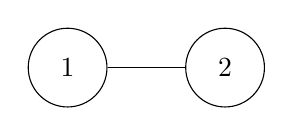
\begin{tikzpicture}
        \tikzstyle{every node}=[draw, circle, minimum size=10mm, inner sep=0pt]
        \node (A) at (0,0) {1};
        \node (B) at (2,0) {2};
        \draw (A) to (B);
    \end{tikzpicture}
\end{center}
\subsection{Analytical}
\noindent The graph is represented by the Hamiltonian
\begin{equation}
    H=-J\begin{pmatrix}
        0&1\\
        1&0
    \end{pmatrix}
\end{equation}
This Hamiltonian indicates that the probability amplitude can "hop" between the two nodes.
We then need to find the eigenvalues of $H$:
\begin{align}
    \begin{vmatrix}
        -\lambda&-J\\
        -J&-\lambda
    \end{vmatrix}=&0\nonumber\\
    \lambda^2-J^2=&0\nonumber\\
    \lambda_1=J\;&\;\;\lambda_2=-J
\end{align}
and their eigenvectors are
\begin{equation}
    u_1=\frac{1}{\sqrt{2}}\begin{pmatrix}
        1\\
        1
    \end{pmatrix}\quad u_2=\frac{1}{\sqrt{2}}\begin{pmatrix}
        1\\
        -1
    \end{pmatrix}
\end{equation}
The time evolution of the quantum state is given by
\begin{equation}
    \label{eq:evolution}
    \ket{\psi(t)}=e^{-\nicefrac{iHt}{\hbar}}\ket{\psi(0)}
\end{equation}
We know that $H$ can be decomposed to
\begin{equation}
    \label{eq:hamiltonian spectral decomposition}
    H=\lambda_1\ket{u_1}\bra{u_1}+\lambda_2\ket{u_2}\bra{u_2}
\end{equation}
By the approximation $e^x=\sum_{n=0}^\infty\nicefrac{x^n}{n!}$, we have
\begin{equation}
    \label{eq:exponential spectral decomposition}
    e^{-\nicefrac{iHt}{\hbar}}=e^{-\nicefrac{i\lambda_1t}{\hbar}}\ket{u_1}\bra{u_1}+e^{-\nicefrac{i\lambda_2t}{\hbar}}\ket{u_2}\bra{u_2}
\end{equation}
The proof of Eq.~\ref{eq:exponential spectral decomposition} can be found in the appendix. To solve for $t$ in Eq.~\ref{eq:evolution}, we still need $\ket{\psi(0)}$ and $\ket{\psi(t)}$. Assuming that the initial state is localised on node 1, we have
\begin{equation}
    \label{eq:initial state}
    \ket{\psi(0)}=\begin{pmatrix}
        1\\
        0
    \end{pmatrix}
\end{equation}
For a perfect quantum state transfer, the final state should be localised on node 2, so
\begin{equation}
    \label{eq:final state}
    \ket{\psi(t)}=\begin{pmatrix}
        0\\
        1
    \end{pmatrix}
\end{equation}
Putting Eq.~\ref{eq:exponential spectral decomposition}, Eq.~\ref{eq:initial state} and Eq.~\ref{eq:final state} into Eq.~\ref{eq:evolution}, we have
\begin{align}
    \begin{pmatrix}
        0\\
        1
    \end{pmatrix}=&\left(e^{-\nicefrac{i\lambda_1t}{\hbar}}\ket{u_1}\bra{u_1}+e^{-\nicefrac{i\lambda_2t}{\hbar}}\ket{u_2}\bra{u_2}\right)\begin{pmatrix}
        1\\
        0
    \end{pmatrix}\nonumber\\
    \begin{pmatrix}
        0\\
        1
    \end{pmatrix}=&\left[e^{-\nicefrac{iJt}{\hbar}}\begin{pmatrix}
        \nicefrac{1}{\sqrt{2}}\\
        \nicefrac{1}{\sqrt{2}}
    \end{pmatrix}\begin{pmatrix}
        \nicefrac{1}{\sqrt{2}}&\nicefrac{1}{\sqrt{2}}
    \end{pmatrix}+e^{\nicefrac{iJt}{\hbar}}\begin{pmatrix}
        \nicefrac{1}{\sqrt{2}}\\
        -\nicefrac{1}{\sqrt{2}}
    \end{pmatrix}\begin{pmatrix}
        \nicefrac{1}{\sqrt{2}}&-\nicefrac{1}{\sqrt{2}}
    \end{pmatrix}\right]\begin{pmatrix}
        1\\
        0
    \end{pmatrix}\nonumber\\
    \begin{pmatrix}
        0\\
        1
    \end{pmatrix}=&\left[e^{-\nicefrac{iJt}{\hbar}}\begin{pmatrix}
        \nicefrac{1}{2}&\nicefrac{1}{2}\\
        \nicefrac{1}{2}&\nicefrac{1}{2}
    \end{pmatrix}+e^{\nicefrac{iJt}{\hbar}}\begin{pmatrix}
        \nicefrac{1}{2}&-\nicefrac{1}{2}\\
        -\nicefrac{1}{2}&\nicefrac{1}{2}
    \end{pmatrix}\right]\begin{pmatrix}
        1\\
        0
    \end{pmatrix}\nonumber\\
    \begin{pmatrix}
        0\\
        1
    \end{pmatrix}=&\begin{pmatrix}
        \nicefrac{e^{-\nicefrac{iJt}{\hbar}}+e^{\nicefrac{iJt}{\hbar}}}{2}&\nicefrac{e^{-\nicefrac{iJt}{\hbar}}-e^{\nicefrac{iJt}{\hbar}}}{2}\\
        \nicefrac{e^{-\nicefrac{iJt}{\hbar}}-e^{\nicefrac{iJt}{\hbar}}}{2}&\nicefrac{e^{-\nicefrac{iJt}{\hbar}}+e^{\nicefrac{iJt}{\hbar}}}{2}
    \end{pmatrix}\begin{pmatrix}
        1\\
        0
    \end{pmatrix}\nonumber\\
    \begin{pmatrix}
        0\\
        1
    \end{pmatrix}=&\begin{pmatrix}
        \nicefrac{e^{-\nicefrac{iJt}{\hbar}}+e^{\nicefrac{iJt}{\hbar}}}{2}\\
        \nicefrac{e^{-\nicefrac{iJt}{\hbar}}-e^{\nicefrac{iJt}{\hbar}}}{2}
    \end{pmatrix}\nonumber\\
    \begin{pmatrix}
        0\\
        1
    \end{pmatrix}=&\begin{pmatrix}
        \cos{\frac{Jt}{\hbar}}\\
        -i\sin{\frac{Jt}{\hbar}}
    \end{pmatrix}\nonumber\\
    t=&\frac{1}{2}\frac{\pi\hbar}{J}
\end{align}
Therefore, the quantum state at node $1$ is transferred to node $2$ with perfect fidelity after $\frac{\pi\hbar}{2J}$ seconds.
To make it dimensionless, we can define the dimensionless time as
\begin{equation}
    t=a\Tilde{t}
\end{equation}
where
\begin{equation}
    a=\frac{\hbar}{J}
\end{equation}
The dimensionless time in this case is
\begin{equation}
    \Tilde{t}=\frac{t}{a}=\frac{\pi\hbar}{2J}\frac{J}{\hbar}=\frac{\pi}{2}
\end{equation}
\subsection{Numerical}
\begin{center}
    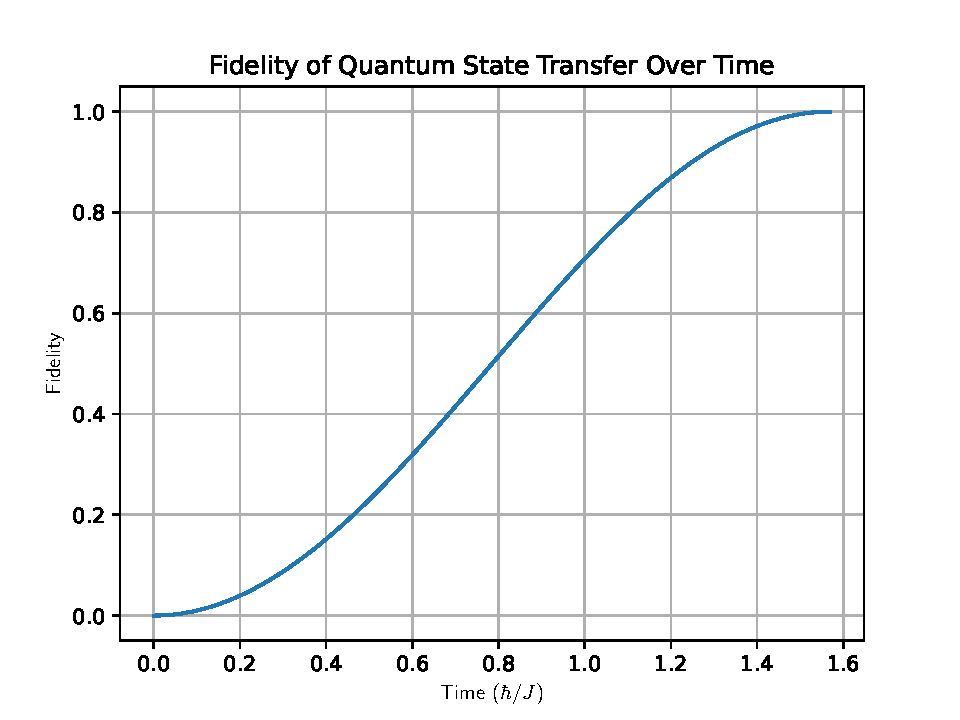
\includegraphics[width=0.7\textwidth]{1d simple linear chain 2 nodes.pdf}
\end{center}
The dimensionless time calculated is
\begin{equation}
    \Tilde{t}=1.5698
\end{equation}
\section{P$_3$}
\begin{center}
    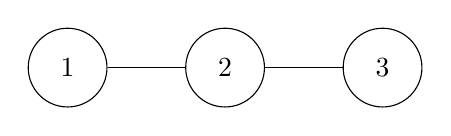
\begin{tikzpicture}
    % Draw nodes
    \node[circle, draw, fill=white, minimum size=1cm] (1) at (0,0) {1};
    \node[circle, draw, fill=white, minimum size=1cm] (2) at (2,0) {2};
    \node[circle, draw, fill=white, minimum size=1cm] (3) at (4,0) {3};
    
    % Draw connections
    \draw[-] (1) -- (2);
    \draw[-] (2) -- (3);
    
    % Labels
    \node[below] at (1) {};
    \node[below] at (2) {};
    \node[below] at (3) {};
\end{tikzpicture}
\end{center}
\subsection{Analytical}
\noindent The graph is represented by the Hamiltonian
\begin{equation}
    H=-J\begin{pmatrix}
        0&1&0\\
        1&0&1\\
        0&1&0
    \end{pmatrix}
\end{equation}
We then need to find the eigenvalues of $H$:
\begin{align}
    \begin{vmatrix}
        -\lambda&-J&0\\
        -J&-\lambda&-J\\
        0&-J&-\lambda
    \end{vmatrix}=&0\nonumber\\
    (-\lambda)(\lambda^2-J^2)+J^2=&0\nonumber\\
    -\lambda^3+2\lambda J^2=&0\nonumber\\
    \lambda(\lambda^2-2J^2)=&0\nonumber\\
    \lambda_1=0\quad\lambda=&\sqrt{2}J\quad\lambda_3=-\sqrt{2}J
\end{align}
and their eigenvectors are
\begin{equation}
    u_1=\frac{1}{\sqrt{2}}\begin{pmatrix}
        1\\
        0\\
        -1
    \end{pmatrix}\quad u_2=\frac{1}{2}\begin{pmatrix}
        1\\
        \sqrt{2}\\
        1
    \end{pmatrix}\quad u_3=\frac{1}{2}\begin{pmatrix}
        1\\
        -\sqrt{2}\\
        1
    \end{pmatrix}
\end{equation}
Assuming the initial state is localised on node 1, we have
\begin{equation}
    \ket{\psi(0)}=\begin{pmatrix}
        1\\
        0\\
        0
    \end{pmatrix}
\end{equation}
For a perfect quantum state transfer, the final state should be localised on node 2, so
\begin{equation}
    \ket{\psi(t)}=\begin{pmatrix}
        0\\
        0\\
        1
    \end{pmatrix}
\end{equation}
Now, we have
\begin{align}
    \begin{pmatrix}
        0\\
        0\\
        1
    \end{pmatrix}=&\left(e^{-\nicefrac{i\lambda_1t}{\hbar}}\ket{u_1}\bra{u_1}+e^{-\nicefrac{i\lambda_2t}{\hbar}}\ket{u_2}\bra{u_2}+e^{-\nicefrac{i\lambda^3t}{\hbar}}\ket{u_3}\bra{u_3}\right)\begin{pmatrix}
        1\\
        0\\
        0
    \end{pmatrix}\nonumber\\
    \begin{pmatrix}
        0\\
        0\\
        1
    \end{pmatrix}=&\left[\begin{pmatrix}
        \nicefrac{1}{\sqrt{2}}\\
        0\\
        -\nicefrac{1}{\sqrt{2}}
    \end{pmatrix}\begin{pmatrix}
        \nicefrac{1}{\sqrt{2}}&0&-\nicefrac{1}{\sqrt{2}}
    \end{pmatrix}+e^{-\nicefrac{i\sqrt{2}Jt}{\hbar}}\begin{pmatrix}
        \nicefrac{1}{2}\\
        \nicefrac{1}{\sqrt{2}}\\
        \nicefrac{1}{2}
    \end{pmatrix}\begin{pmatrix}
        \nicefrac{1}{2}&\nicefrac{1}{\sqrt{2}}&\nicefrac{1}{2}
    \end{pmatrix}+e^{\nicefrac{i\sqrt{2}Jt}{\hbar}}\begin{pmatrix}
        \nicefrac{1}{2}\\
        -\nicefrac{1}{\sqrt{2}}\\
        \nicefrac{1}{2}
    \end{pmatrix}\begin{pmatrix}
        \nicefrac{1}{2}&-\nicefrac{1}{\sqrt{2}}&\nicefrac{1}{2}
    \end{pmatrix}\right]\nonumber\\
    \begin{pmatrix}
        0\\
        0\\
        1
    \end{pmatrix}=&\left[\begin{pmatrix}
        \nicefrac{1}{2}&0&-\nicefrac{1}{2}\\
        0&0&0\\
        -\nicefrac{1}{2}&0&\nicefrac{1}{2}
    \end{pmatrix}+e^{-\nicefrac{i\sqrt{2}t}{\hbar}}\begin{pmatrix}
        \nicefrac{1}{4}&\nicefrac{1}{2\sqrt{2}}&\nicefrac{1}{4}\\
        \nicefrac{1}{2\sqrt{2}}&\nicefrac{1}{2}&\nicefrac{1}{2\sqrt{2}}\\
        \nicefrac{1}{4}&\nicefrac{1}{2\sqrt{2}}&\nicefrac{1}{4}
    \end{pmatrix}+e^{\nicefrac{i\sqrt{2}Jt}{\hbar}}\begin{pmatrix}
        \nicefrac{1}{4}&-\nicefrac{1}{2\sqrt{2}}&\nicefrac{1}{4}\\
        -\nicefrac{1}{2\sqrt{2}}&\nicefrac{1}{2}&-\nicefrac{1}{2\sqrt{2}}\\
        \nicefrac{1}{4}&-\nicefrac{1}{2\sqrt{2}}&\nicefrac{1}{4}
    \end{pmatrix}\right]\begin{pmatrix}
        1\\
        0\\
        0
    \end{pmatrix}\nonumber\\
    \begin{pmatrix}
        0\\
        0\\
        1
    \end{pmatrix}=&\begin{pmatrix}
        \left(\nicefrac{1}{2}+\nicefrac{e^{-\nicefrac{i\sqrt{2}Jt}{\hbar}}}{4}+\nicefrac{e^{\nicefrac{i\sqrt{2}Jt}{\hbar}}}{4}\right)&\left(\nicefrac{e^{-\nicefrac{i\sqrt{2}Jt}{\hbar}}}{2\sqrt{2}}-\nicefrac{e^{\nicefrac{i\sqrt{2}Jt}{\hbar}}}{2\sqrt{2}}\right)&\left(-\nicefrac{1}{2}+\nicefrac{e^{-\nicefrac{i\sqrt{2}Jt}{\hbar}}}{4}+\nicefrac{e^{\nicefrac{i\sqrt{2}Jt}{\hbar}}}{4}\right)\\
        \left(\nicefrac{e^{-\nicefrac{i\sqrt{2}Jt}{\hbar}}}{2\sqrt{2}}-\nicefrac{e^{\nicefrac{i\sqrt{2}Jt}{\hbar}}}{2\sqrt{2}}\right)&\left(\nicefrac{e^{-\nicefrac{i\sqrt{2}Jt}{\hbar}}}{2}+\nicefrac{e^{\nicefrac{i\sqrt{2}Jt}{\hbar}}}{2}\right)&\left(\nicefrac{e^{-\nicefrac{i\sqrt{2}Jt}{\hbar}}}{2\sqrt{2}}-\nicefrac{e^{\nicefrac{i\sqrt{2}Jt}{\hbar}}}{2\sqrt{2}}\right)\\
        \left(-\nicefrac{1}{2}+\nicefrac{e^{-\nicefrac{i\sqrt{2}Jt}{\hbar}}}{4}+\nicefrac{e^{\nicefrac{i\sqrt{2}Jt}{\hbar}}}{4}\right)&\left(\nicefrac{e^{-\nicefrac{i\sqrt{2}Jt}{\hbar}}}{2\sqrt{2}}-\nicefrac{e^{\nicefrac{i\sqrt{2}Jt}{\hbar}}}{2\sqrt{2}}\right)&\left(\nicefrac{1}{2}+\nicefrac{e^{-\nicefrac{i\sqrt{2}Jt}{\hbar}}}{4}+\nicefrac{e^{\nicefrac{i\sqrt{2}Jt}{\hbar}}}{4}\right)
    \end{pmatrix}\begin{pmatrix}
        1\\
        0\\
        0
    \end{pmatrix}\nonumber\\
    \begin{pmatrix}
        0\\
        0\\
        1
    \end{pmatrix}=&\begin{pmatrix}
        \nicefrac{1}{2}+\nicefrac{e^{-\nicefrac{i\sqrt{2}Jt}{\hbar}}}{4}+\nicefrac{e^{\nicefrac{i\sqrt{2}Jt}{\hbar}}}{4}\\
        \nicefrac{e^{-\nicefrac{i\sqrt{2}Jt}{\hbar}}}{2\sqrt{2}}-\nicefrac{e^{\nicefrac{i\sqrt{2}Jt}{\hbar}}}{2\sqrt{2}}\\
        -\nicefrac{1}{2}+\nicefrac{e^{-\nicefrac{i\sqrt{2}Jt}{\hbar}}}{4}+\nicefrac{e^{\nicefrac{i\sqrt{2}Jt}{\hbar}}}{4}
    \end{pmatrix}\nonumber\\
    \begin{pmatrix}
        0\\
        0\\
        1
    \end{pmatrix}=&\begin{pmatrix}
        \frac{1}{2} \left( 1 + \cos \left( \frac{\sqrt{2} J t}{\hbar} \right) \right) \\
        -\frac{i}{\sqrt{2}} \sin \left( \frac{\sqrt{2} J t}{\hbar} \right) \\
        \frac{1}{2} \left( -1 + \cos \left( \frac{\sqrt{2} J t}{\hbar} \right) \right)
    \end{pmatrix}\nonumber\\
    t=&\frac{\pi\hbar}{\sqrt{2}J}
\end{align}
or in dimensionless terms,
\begin{equation}
    \Tilde{t}=\frac{\pi}{\sqrt{2}}
\end{equation}
\subsection{Numerical}
\begin{center}
    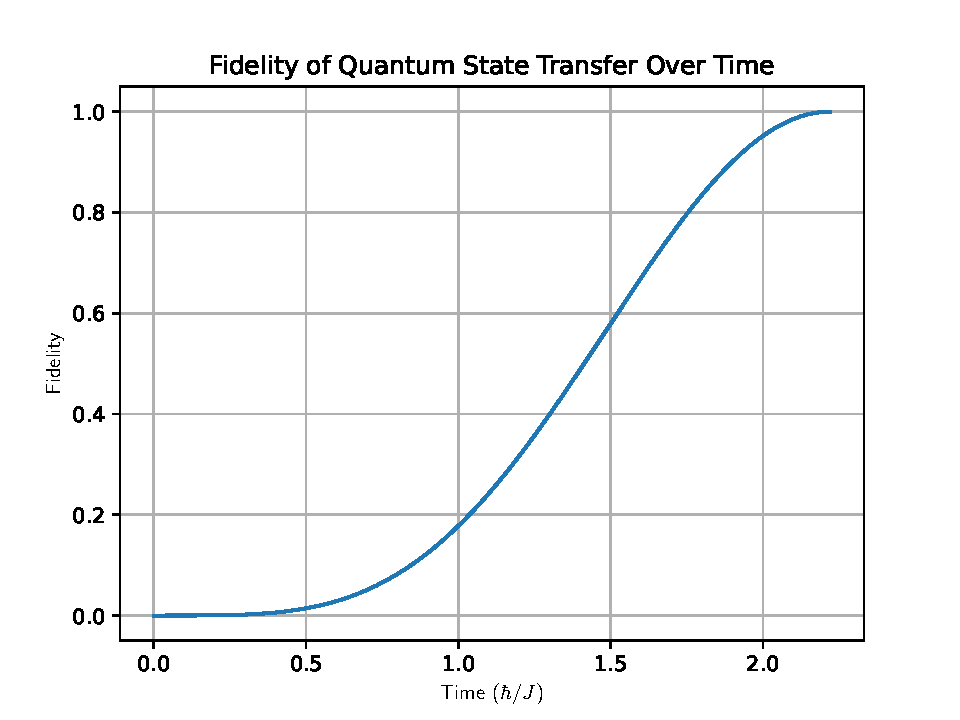
\includegraphics[width=0.7\textwidth]{1d simple linear chain 3 nodes.pdf}
\end{center}
The dimensionless calculated is
\begin{equation}
    \Tilde{t}=2.2205
\end{equation}
which agrees with the analytical result.
\section{P$_4$}
\begin{center}
    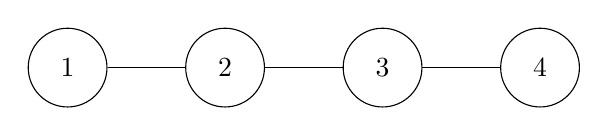
\begin{tikzpicture}
    % Draw nodes
    \node[circle, draw, fill=white, minimum size=1cm] (1) at (0,0) {1};
    \node[circle, draw, fill=white, minimum size=1cm] (2) at (2,0) {2};
    \node[circle, draw, fill=white, minimum size=1cm] (3) at (4,0) {3};
    \node[circle, draw, fill=white, minimum size=1cm] (4) at (6,0) {4};
    
    % Draw connections
    \draw[-] (1) -- (2);
    \draw[-] (2) -- (3);
    \draw[-] (3) -- (4);
    
    % Labels
    \node[below] at (1) {};
    \node[below] at (2) {};
    \node[below] at (3) {};
    \node[below] at (4) {};
\end{tikzpicture}
\end{center}
\subsection{Analytical}
\noindent The graph is represented by the Hamiltonian
\begin{equation}
    H=-J\begin{pmatrix}
        0&1&0&0\\
        1&0&1&0\\
        0&1&0&1\\
        0&0&1&0
    \end{pmatrix}
\end{equation}
Using Mathematica, the eigenvalues are found to be
\begin{equation}
    \lambda_1=\frac{J}{2}(-1-\sqrt{5})\quad\lambda_2=\frac{J}{2}(1+\sqrt{5})\quad\lambda_3=\frac{J}{2}(1-\sqrt{5})\quad\lambda_4=\frac{J}{2}(-1+\sqrt{5})
\end{equation}
and their eigenvectors are
\begin{equation}
    u_1=\begin{pmatrix}
        1\\
        \frac{1}{2}(1+\sqrt{5})\\
        \frac{1}{2}(1+\sqrt{5})\\
        1
    \end{pmatrix}\quad u_2=\begin{pmatrix}
        -1\\
        \frac{1}{2}(1+\sqrt{5})\\
        \frac{1}{2}(-1-\sqrt{5})\\
        1
    \end{pmatrix}\quad u_3=\begin{pmatrix}
        -1\\
        \frac{1}{2}(1-\sqrt{5})\\
        \frac{1}{2}(-1+\sqrt{5})\\
        1
    \end{pmatrix}\quad u_4=\begin{pmatrix}
        1\\
        \frac{1}{2}(1-\sqrt{5})\\
        \frac{1}{2}(1-\sqrt{5})\\
        1
    \end{pmatrix}
\end{equation}
\subsection{Numerical}
\noindent Assuming the initial state is localised on node 1, we have
\begin{equation}
    \ket{\psi(0)}=\begin{pmatrix}
        1\\
        0\\
        0\\
        0
    \end{pmatrix}
\end{equation}
I am not sure about what the target state should be, so I tried different cases.
\begin{itemize}
    \item When the target state is
    \begin{equation}
        \ket{\psi(t)}=\begin{pmatrix}
            0\\
            1\\
            0\\
            0
        \end{pmatrix}
    \end{equation}
    \begin{center}
        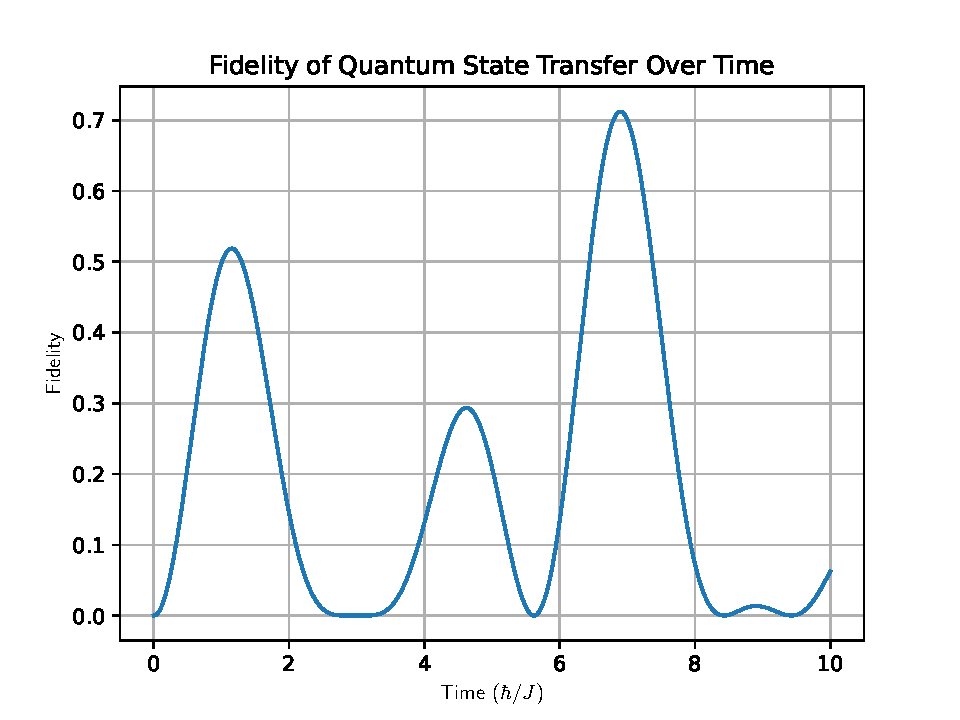
\includegraphics[width=0.7\textwidth]{1d simple linear chain 4 nodes (2).pdf}
    \end{center}
    \item When the target state is
    \begin{equation}
        \ket{\psi(t)}=\begin{pmatrix}
            0\\
            0\\
            1\\
            0
        \end{pmatrix}
    \end{equation}
    \begin{center}
        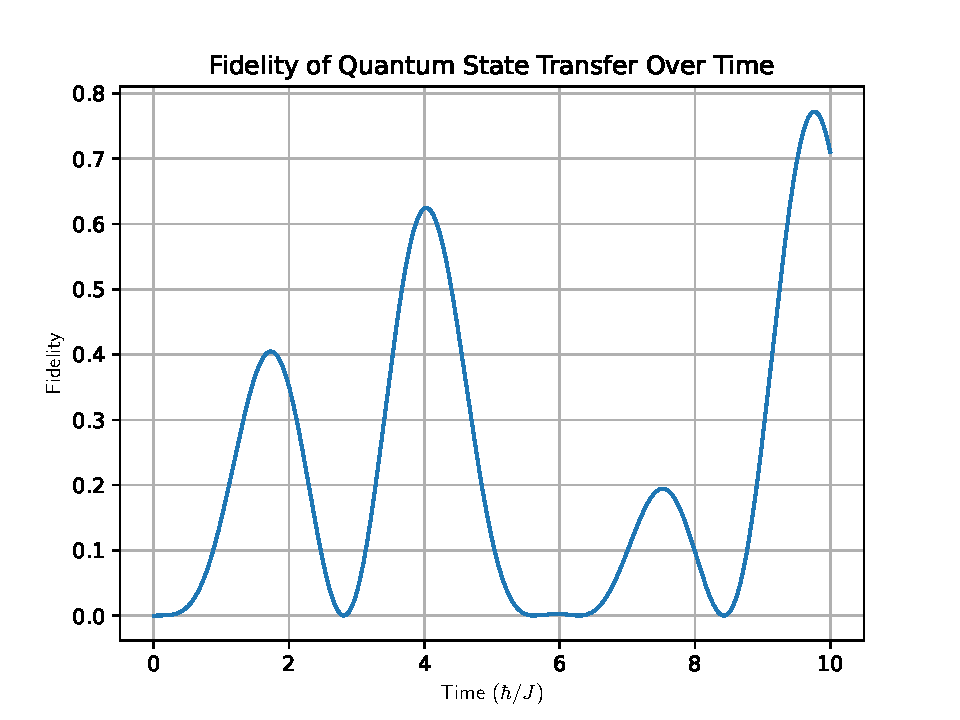
\includegraphics[width=0.7\textwidth]{1d simple linear chain 4 nodes (3).pdf}
    \end{center}
    \item When the target state is
    \begin{equation}
        \ket{\psi(t)}=\begin{pmatrix}
            0\\
            0\\
            0\\
            1
        \end{pmatrix}
    \end{equation}
    \begin{center}
        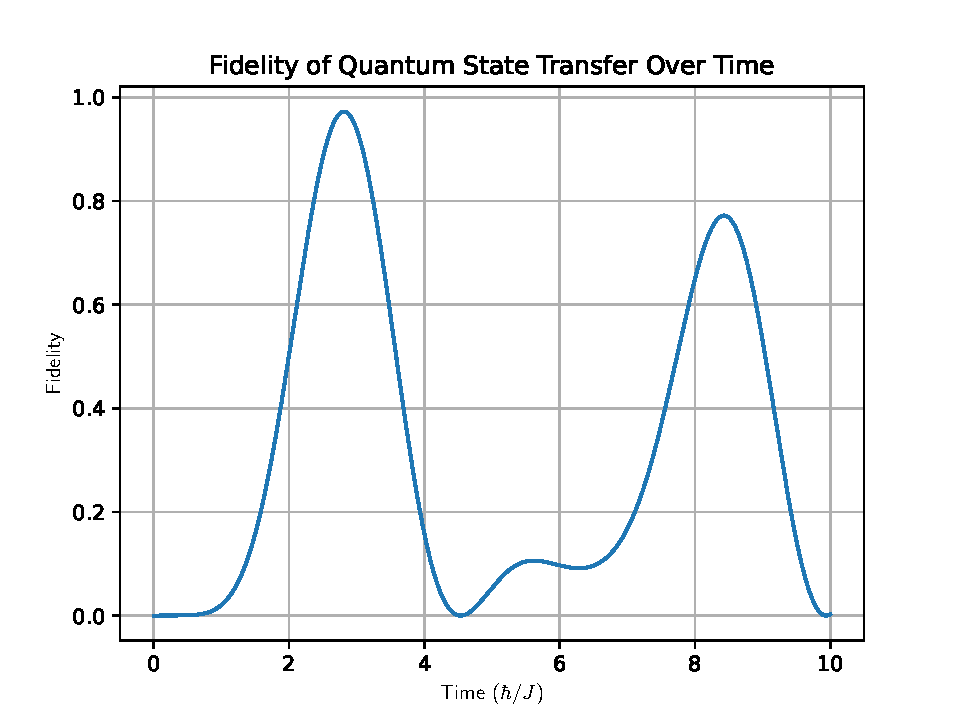
\includegraphics[width=0.7\textwidth]{1d simple linear chain 4 nodes (4).pdf}
    \end{center}
\end{itemize}
We can see that in the first $10$ seconds, although a high-fidelity transfer can take place from node 1 to node 4, it is not a perfect quantum state transfer.
\section{C$_4$}
\begin{center}
    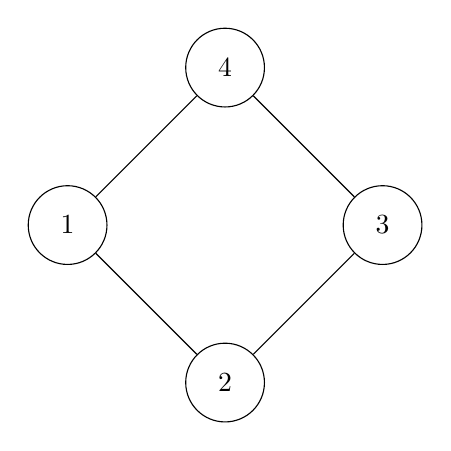
\begin{tikzpicture}
    % Define positions of the nodes in a square (cycle)
    \node[circle, draw, fill=white, minimum size=1cm] (1) at (0, 2) {1};
    \node[circle, draw, fill=white, minimum size=1cm] (2) at (2, 0) {2};
    \node[circle, draw, fill=white, minimum size=1cm] (3) at (4, 2) {3};
    \node[circle, draw, fill=white, minimum size=1cm] (4) at (2, 4) {4};

    % Draw edges between consecutive nodes
    \draw[-] (1) -- (2);
    \draw[-] (2) -- (3);
    \draw[-] (3) -- (4);
    \draw[-] (4) -- (1);

    % Optional: add labels
    \node[below left] at (1) {};
    \node[below right] at (2) {};
    \node[below right] at (3) {};
    \node[above] at (4) {};
\end{tikzpicture}
\end{center}
\subsection{Analytical}
\noindent The graph is represented by the Hamiltonian
\begin{equation}
    H=-J\begin{pmatrix}
        0&1&0&1\\
        1&0&1&0\\
        0&1&0&1\\
        1&0&1&0
    \end{pmatrix}
\end{equation}
Using Mathematica, the eigenvalues are found to be
\begin{equation}
    \lambda_1=-J\sqrt{3}\quad\lambda_2=J\sqrt{3}\quad\lambda_3=0\quad\lambda_4=0
\end{equation}
and their eigenvectors are
\begin{equation}
    u_1=\begin{pmatrix}
        \frac{1}{\sqrt{3}}\\
        1\\
        \frac{2}{\sqrt{3}}\\
        1
    \end{pmatrix}\quad u_2=\begin{pmatrix}
        -\frac{1}{\sqrt{3}}\\
        1\\
        -\frac{2}{\sqrt{3}}\\
        1
    \end{pmatrix}\quad u_3=\begin{pmatrix}
        -1\\
        0\\
        1\\
        0
    \end{pmatrix}\quad u_4=\begin{pmatrix}
        0\\
        0\\
        0\\
        0
    \end{pmatrix}
\end{equation}
\subsection{Numerical}
\noindent Assuming the initial state is localised on node $1$, we have
\begin{equation}
    \ket{\psi(0)}=\begin{pmatrix}
        1\\
        0\\
        0\\
        0
    \end{pmatrix}
\end{equation}
By symmetry, the final state should  be localised on node $3$, so
\begin{equation}
    \ket{\psi(t)}=\begin{pmatrix}
        0\\
        0\\
        1\\
        0
    \end{pmatrix}
\end{equation}
\begin{center}
    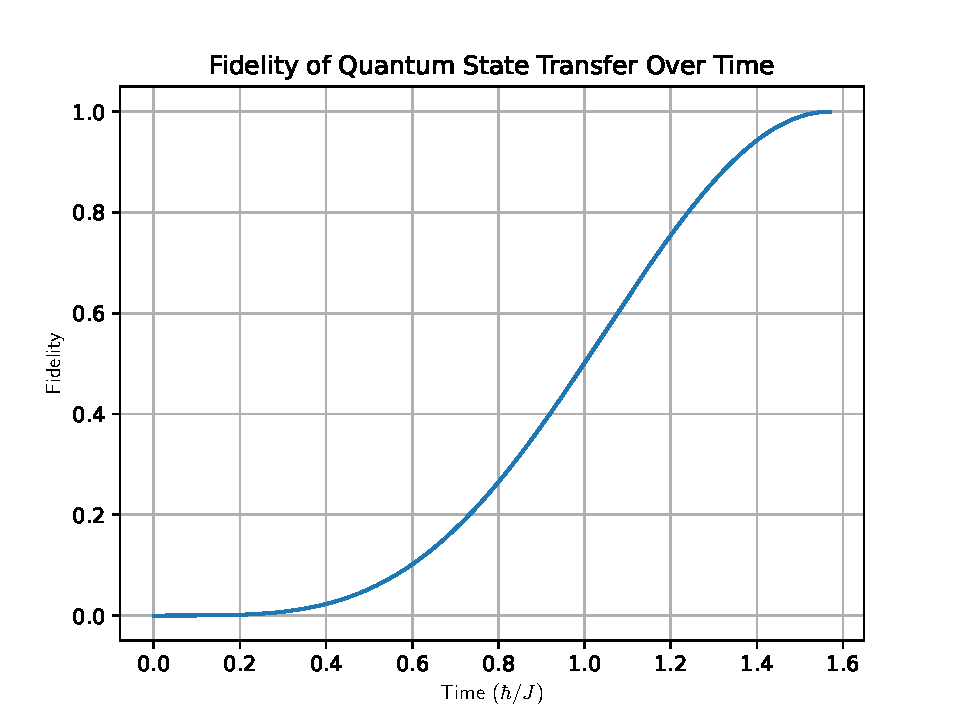
\includegraphics[width=0.7\textwidth]{c_4.pdf}
\end{center}
The calculated dimensionless time is
\begin{equation}
    \Tilde{t}=1.5701
\end{equation}
\section{K$_4$}
\begin{center}
    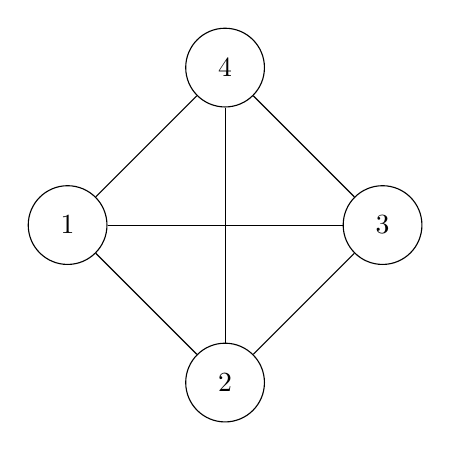
\begin{tikzpicture}
    % Define positions of the nodes
    \node[circle, draw, fill=white, minimum size=1cm] (1) at (0, 2) {1};
    \node[circle, draw, fill=white, minimum size=1cm] (2) at (2, 0) {2};
    \node[circle, draw, fill=white, minimum size=1cm] (3) at (4, 2) {3};
    \node[circle, draw, fill=white, minimum size=1cm] (4) at (2, 4) {4};

    % Draw edges between each pair of nodes
    \draw[-] (1) -- (2);
    \draw[-] (1) -- (3);
    \draw[-] (1) -- (4);
    \draw[-] (2) -- (3);
    \draw[-] (2) -- (4);
    \draw[-] (3) -- (4);

    % Optional: add labels
    \node[below left] at (1) {};
    \node[below right] at (2) {};
    \node[below right] at (3) {};
    \node[above] at (4) {};
\end{tikzpicture}
\end{center}
\subsection{Analytical}
\noindent The graph is represented by the Hamiltonian
\begin{equation}
    H=-J\begin{pmatrix}
        0&1&1&1\\
        1&0&1&1\\
        1&1&0&1\\
        1&1&1&0
    \end{pmatrix}
\end{equation}
Using Mathematica, the eigenvalues are found to be
\begin{equation}
    \lambda_1=-3J\quad\lambda_2=J\quad\lambda_3=J\quad\lambda_4=J
\end{equation}
and their eigenvectors are
\begin{equation}
    u_1=\begin{pmatrix}
        1\\
        1\\
        1\\
        1
    \end{pmatrix}\quad u_2=\begin{pmatrix}
        -1\\
        0\\
        0\\
        1
    \end{pmatrix}\quad u_3=\begin{pmatrix}
        -1\\
        0\\
        1\\
        0
    \end{pmatrix}\quad u_4=\begin{pmatrix}
        -1\\
        1\\
        0\\
        0
    \end{pmatrix}
\end{equation}
\subsection{Numerical}
\noindent Assuming the initial state is localised on node $1$, we have
\begin{equation}
    \ket{\psi(0)}=\begin{pmatrix}
        1\\
        0\\
        0\\
        0
    \end{pmatrix}
\end{equation}
I am not sure about what the target state should be, so I tried different cases.
\begin{itemize}
    \item When the target state is
    \begin{equation}
        \ket{\psi(t)}=\begin{pmatrix}
            0\\
            0\\
            0\\
            1
        \end{pmatrix}
    \end{equation}
    \begin{center}
        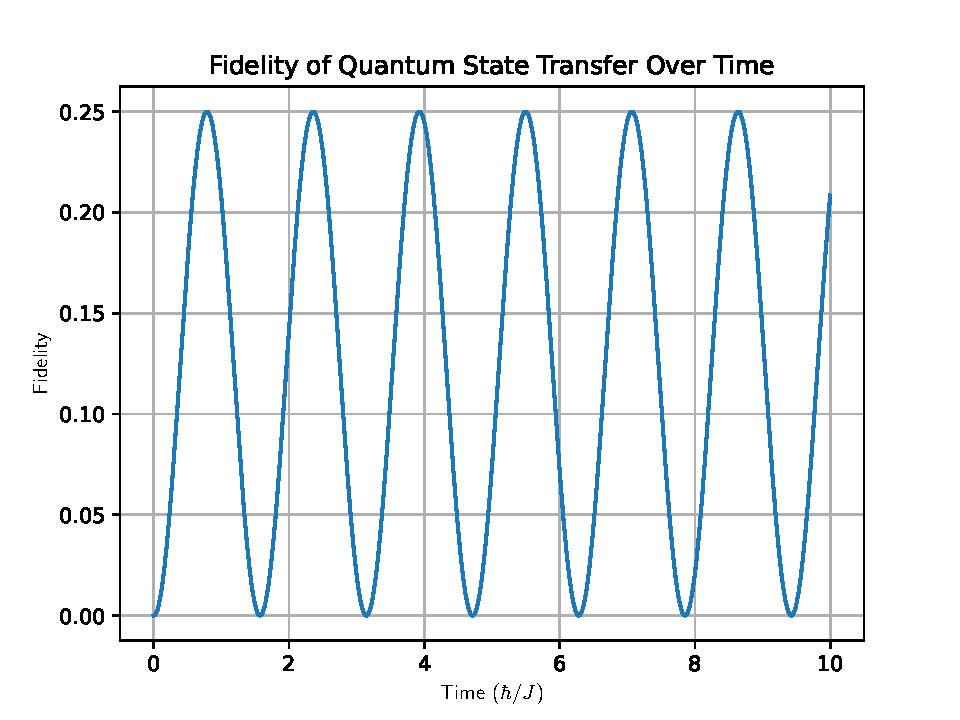
\includegraphics[width=0.7\textwidth]{k_4 (2).pdf}
    \end{center}
    \item When the target state is
    \begin{equation}
        \ket{\psi(t)}=\begin{pmatrix}
            0\\
            0\\
            1\\
            0
        \end{pmatrix}
    \end{equation}
    \begin{center}
        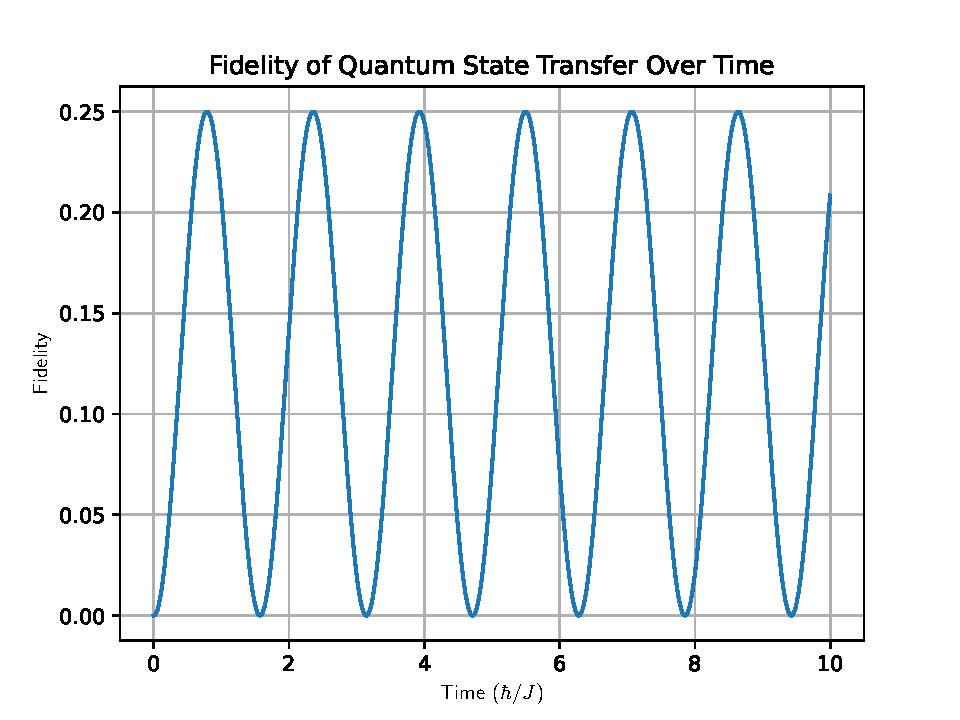
\includegraphics[width=0.7\textwidth]{k_4 (3).pdf}
    \end{center}
    \item When the target state is
    \begin{equation}
        \ket{\psi(t)}=\begin{pmatrix}
            0\\
            0\\
            0\\
            1
        \end{pmatrix}
    \end{equation}
    \begin{center}
        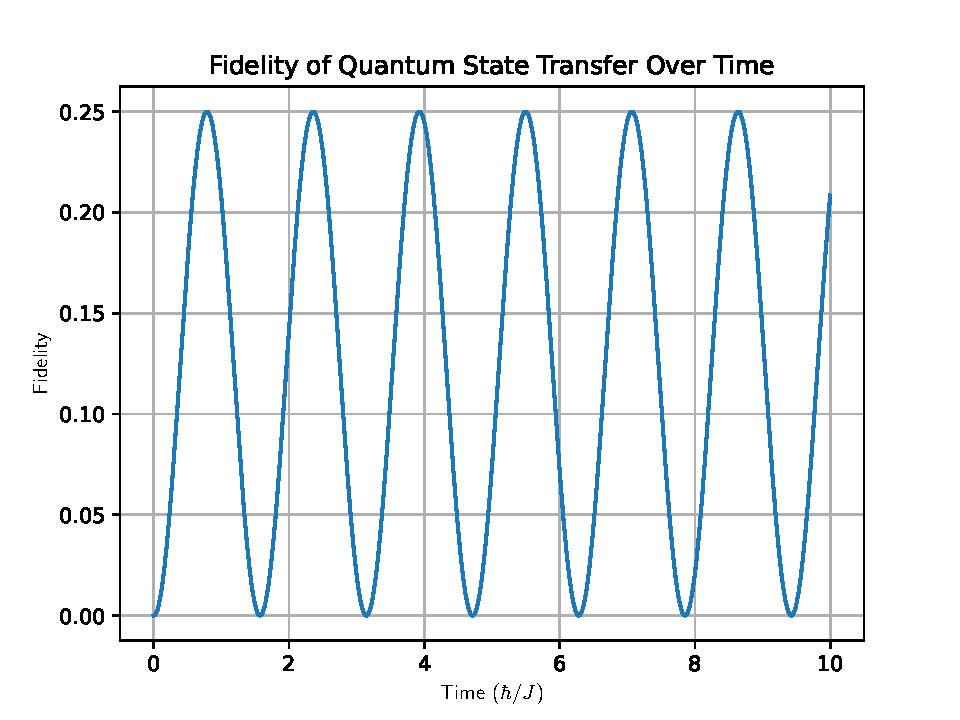
\includegraphics[width=0.7\textwidth]{k_4 (4).pdf}
    \end{center}
\end{itemize}
We can see that one step perfect quantum state transfer does not take place in the first $10$ seconds.
\section{Conclusion}
\noindent In summary, we conjecture that for a graph to allow one-step perfect quantum state transfer (PST), its eigenvalues must include a term proportional to \( \sqrt{n - 1} \), where \( n \) is the number of nodes in the graph. This condition on the eigenvalues suggests a specific energy spacing that facilitates the oscillation required for state transfer between nodes. For a particular class of graphs, such as the \( P \)-graphs that meet this eigenvalue condition, the time needed for one-step PST can be expressed as \( \tilde{t} = \nicefrac{\pi}{\lambda_{\text{max}}} \), where \( \lambda_{\text{max}} \) is the largest eigenvalue of the Hamiltonian matrix for the system. This relationship implies that the maximum energy separation in the system's spectrum dictates the speed of state transfer, reinforcing the connection between spectral properties and dynamical behavior in quantum networks.\\
However, it is important to note that this hypothesis is based on a limited set of samples, and more comprehensive testing across a wider variety of graphs is needed to confirm its general validity. Further exploration may provide additional insights or reveal exceptions to this conjecture.
\section{Conditions for Perfect Quantum State Transfer and Periodicity in Graph}
\subsection{Necessary Conditions for PST}
These conditions are required for PST to occur, meaning PST cannot happen without them.
\begin{enumerate}
    \item Let $u_1,...,u_m$ be the eigenvectors in the spectral decomposition of $A(X)$ and let $\lambda_1,...,\lambda_m$ be the corresponding eigenvalues, then there is perfect quantum state transform from $\alpha$ to $\beta$ at time $\tau$ if and only if there is constant $\gamma$ such that
    \begin{equation}
        u_r|\alpha\rangle=\gamma\exp{(-i\tau\lambda_r)}u_r|\beta\rangle\quad(r=1,...,m)
    \end{equation}
\end{enumerate}
\subsection{Sufficient Conditions for PST}
These conditions ensure PST but are not strictly required.
\begin{enumerate}
    \item If we have perfect quantum state transfer on $X$ from $\alpha$ to $\beta$ at time $\tau$, then we must have perfect quantum state transfer from $\beta$ to $\alpha$ at the same time $\tau$.
    \item Suppose $X$ is a connected graph and $X$ is periodic at $\alpha$ with minimum period $\sigma$. Then if there is perfect quantum state transfer from $\alpha$ to $\beta$, then there must be perfect quantum state transfer from $\beta$ to $\alpha$ at time $\nicefrac{\sigma}{2}$.
    \item If we have perfect quantum state transfer from $\alpha$ to $\beta$ in $X$ at time $\tau$, then at time $\tau$ we have perfect quantum state transfer in the $d$th Cartesian power of $X$ between the $d$-tuples.
\end{enumerate}
\subsection{Derived Implications for PST}
These are consequences of PST occurring or supplementary observations about its behavior.
\begin{enumerate}
    \item If we have perfect quantum state transfer on $X$ from $\alpha$ to $\beta$ at time $\tau$, then $X$ must be periodic at $\alpha$ and $\beta$ with period $2\tau$.
    \item If we have perfect quantum state transfer in $X$ from $\alpha$ to $\beta$ and also from $\alpha$ to $\gamma$, then $\beta=\gamma$.
\end{enumerate}
\subsection{Sufficient conditions for Periodicity}
These conditions ensure periodicity but are not strictly required.
\begin{enumerate}
    \item The eigenvalues of $X$ are integers
    \item The eigenvalues of $X$ are rational multipliers of $\sqrt{\Delta}$, for some square-free integer $\Delta$.
    \item If we have perfect quantum state transfer on $X$ from $\alpha$ to $\beta$ at time $\tau$, then $X$ must be periodic at $\alpha$ and $\beta$ with period $2\tau$.
\end{enumerate}
\section{Two-Step PST of P$_4$}
\subsection{Case 1}
\begin{center}
    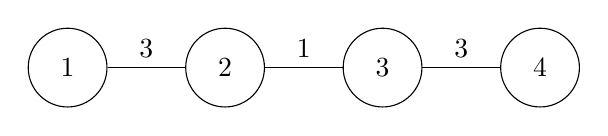
\begin{tikzpicture}
    % Draw nodes
    \node[circle, draw, fill=white, minimum size=1cm] (1) at (0,0) {1};
    \node[circle, draw, fill=white, minimum size=1cm] (2) at (2,0) {2};
    \node[circle, draw, fill=white, minimum size=1cm] (3) at (4,0) {3};
    \node[circle, draw, fill=white, minimum size=1cm] (4) at (6,0) {4};
    
    % Draw connections
    \draw[-] (1) -- (2) node[midway, above] {$3$};
    \draw[-] (2) -- (3) node[midway, above] {$1$};
    \draw[-] (3) -- (4) node[midway, above] {$3$};
    
    % Labels
    \node[below] at (1) {};
    \node[below] at (2) {};
    \node[below] at (3) {};
    \node[below] at (4) {};
\end{tikzpicture}
\end{center}
The initial Hamiltonian is
\begin{equation}
    H=\begin{pmatrix}
        0&3&0&0\\
        3&0&1&0\\
        0&1&0&3\\
        0&0&3&0
    \end{pmatrix}
\end{equation}
The states are
\begin{equation}
    \psi_{initial}=\begin{pmatrix}
        1\\
        0\\
        0\\
        0
    \end{pmatrix},\quad\psi_{target}=\begin{pmatrix}
        0\\
        0\\
        0\\
        1
    \end{pmatrix}
\end{equation}
For two-step perfect quantum state transfer to occur, I evolved the initial state until $\tilde{t}=4.153943$. The fidelity at that time is calculated numerically to be $0.7708606$.
After that, I adjusted the edge weights:
\begin{center}
    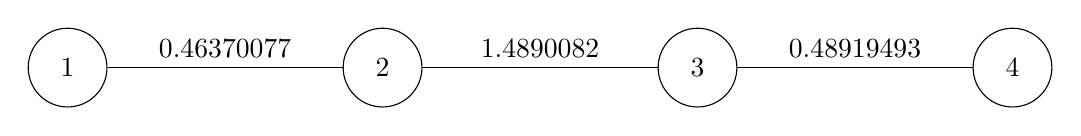
\begin{tikzpicture}
    % Draw nodes
    \node[circle, draw, fill=white, minimum size=1cm] (1) at (0,0) {1};
    \node[circle, draw, fill=white, minimum size=1cm] (2) at (4,0) {2};
    \node[circle, draw, fill=white, minimum size=1cm] (3) at (8,0) {3};
    \node[circle, draw, fill=white, minimum size=1cm] (4) at (12,0) {4};
    
    % Draw connections
    \draw[-] (1) -- (2) node[midway, above] {$0.46370077$};
    \draw[-] (2) -- (3) node[midway, above] {$1.4890082$};
    \draw[-] (3) -- (4) node[midway, above] {$0.48919493$};
    
    % Labels
    \node[below] at (1) {};
    \node[below] at (2) {};
    \node[below] at (3) {};
    \node[below] at (4) {};
\end{tikzpicture}
\end{center}
Then, I evolved the intermediate state, and a fidelity larger than $0.999$ was calculated when
\begin{equation}
    \tilde{t}=7.5220
\end{equation}
\begin{center}
    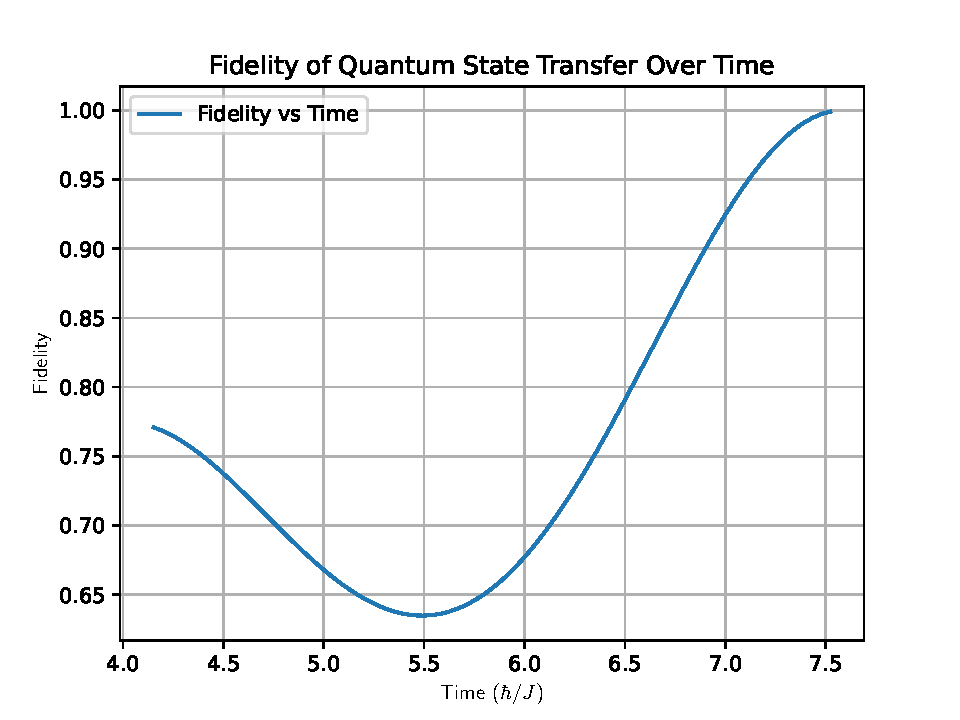
\includegraphics[width=0.7\textwidth]{p_4 two step case 1.pdf}
\end{center}
\subsection{Case 2}
\begin{center}
    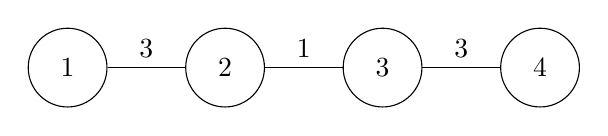
\begin{tikzpicture}
    % Draw nodes
    \node[circle, draw, fill=white, minimum size=1cm] (1) at (0,0) {1};
    \node[circle, draw, fill=white, minimum size=1cm] (2) at (2,0) {2};
    \node[circle, draw, fill=white, minimum size=1cm] (3) at (4,0) {3};
    \node[circle, draw, fill=white, minimum size=1cm] (4) at (6,0) {4};
    
    % Draw connections
    \draw[-] (1) -- (2) node[midway, above] {$3$};
    \draw[-] (2) -- (3) node[midway, above] {$1$};
    \draw[-] (3) -- (4) node[midway, above] {$3$};
    
    % Labels
    \node[below] at (1) {};
    \node[below] at (2) {};
    \node[below] at (3) {};
    \node[below] at (4) {};
\end{tikzpicture}
\end{center}
The initial Hamiltonian is
\begin{equation}
    H=\begin{pmatrix}
        0&3&0&0\\
        3&0&1&0\\
        0&1&0&3\\
        0&0&3&0
    \end{pmatrix}
\end{equation}
The states are
\begin{equation}
    \psi_{initial}=\begin{pmatrix}
        1\\
        0\\
        0\\
        0
    \end{pmatrix},\quad\psi_{target}=\begin{pmatrix}
        0\\
        0\\
        0\\
        1
    \end{pmatrix}
\end{equation}
For two-step perfect quantum state transfer to occur, I evolved the initial state until $\tilde{t}=4.1858525$. The fidelity at that time is calculated numerically to be $0.7542758$.
After that, I adjusted the edge weights:
\begin{center}
    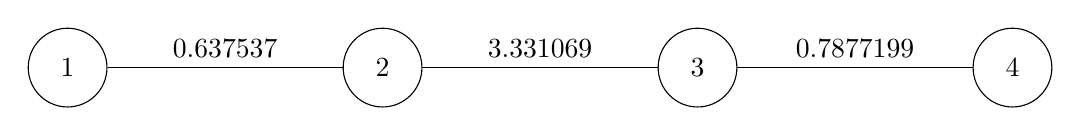
\begin{tikzpicture}
    % Draw nodes
    \node[circle, draw, fill=white, minimum size=1cm] (1) at (0,0) {1};
    \node[circle, draw, fill=white, minimum size=1cm] (2) at (4,0) {2};
    \node[circle, draw, fill=white, minimum size=1cm] (3) at (8,0) {3};
    \node[circle, draw, fill=white, minimum size=1cm] (4) at (12,0) {4};
    
    % Draw connections
    \draw[-] (1) -- (2) node[midway, above] {$0.637537$};
    \draw[-] (2) -- (3) node[midway, above] {$3.331069$};
    \draw[-] (3) -- (4) node[midway, above] {$0.7877199$};
    
    % Labels
    \node[below] at (1) {};
    \node[below] at (2) {};
    \node[below] at (3) {};
    \node[below] at (4) {};
\end{tikzpicture}
\end{center}
Then, I evolved the intermediate state, and a fidelity larger than $0.999$ was calculated when
\begin{equation}
    \tilde{t}=7.4668
\end{equation}
\begin{center}
    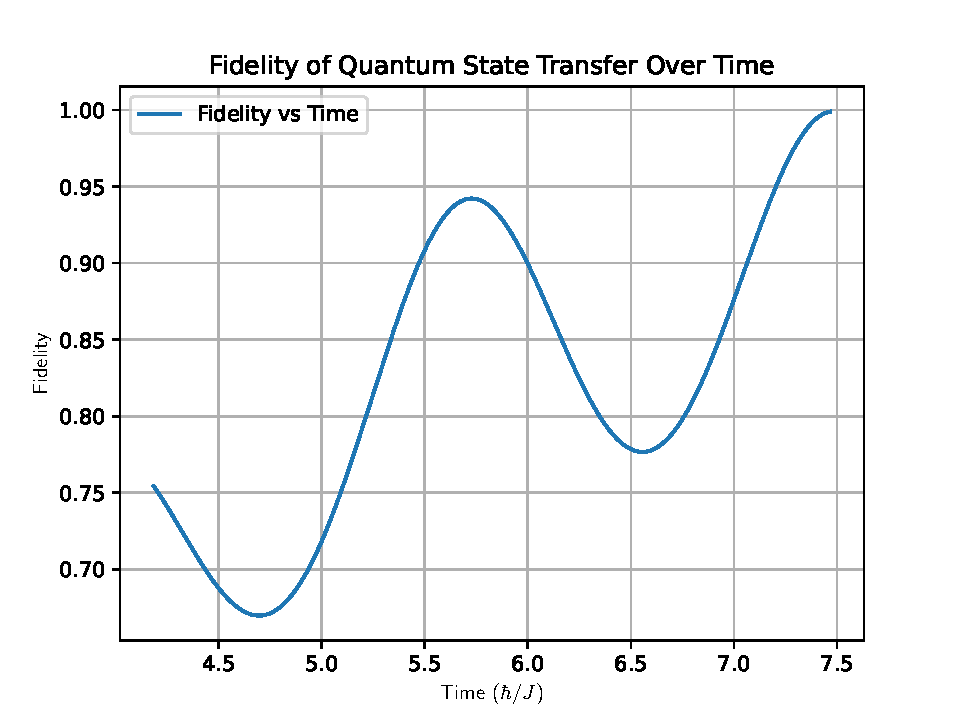
\includegraphics[width=0.7\textwidth]{p_4 two step case 2.pdf}
\end{center}
\section{P$_4$: Validator}
\subsection{Time Evolution of Quantum States in Float64}
\subsubsection{Imports}
Import the required libraries: 
\begin{itemize}
    \item \texttt{numpy} – for numerical operations
    \item \texttt{scipy.linalg.expm} – to compute matrix exponentials
    \item \texttt{matplotlib.pyplot} – for potential plotting (though not used directly)
\end{itemize}

\subsubsection{Fidelity Calculation}
\begin{enumerate}
    \item Compute the time evolution operator:
    \[
    U(t) = e^{-i H t}
    \]
    \item Evolve the initial state:
    \[
    \psi(t) = U(t) \psi_0
    \]
    \item Calculate fidelity:
    \[
    F = \left| \langle \psi_T | \psi(t) \rangle \right|^2
    \]
\end{enumerate}

\subsubsection{Hamiltonian Generation}
\noindent Generate a $4 \times 4$ Hamiltonian for a path graph of four nodes:
\[
H_{ij} = \begin{cases}
w_1 & \text{if } (i, j) = (1, 2) \text{ or } (2, 1) \\
w_2 & \text{if } (i, j) = (2, 3) \text{ or } (3, 2) \\
w_3 & \text{if } (i, j) = (3, 4) \text{ or } (4, 3) \\
0 & \text{otherwise}
\end{cases}
\]

\subsubsection{Main Process}
\begin{enumerate}
    \item Receive user input for:
    \begin{itemize}
        \item Initial edge weights $[w_1, w_2, w_3]$
        \item Final edge weights $[w'_1, w'_2, w'_3]$
        \item Runtime before adjustment $t_1$
        \item Runtime after adjustment $t_2$
    \end{itemize}
    \item Generate the initial and final Hamiltonians:
    \[
    H_1 = H(w), \quad H_2 = H(w')
    \]
    \item Define the initial state (excitation at node 1):
    \[
    \psi_0 = \begin{bmatrix} 1 & 0 & 0 & 0 \end{bmatrix}^T
    \]
    \item Define the target state (excitation at node 3):
    \[
    \psi_T = \begin{bmatrix} 0 & 0 & 1 & 0 \end{bmatrix}^T
    \]
    \item Normalize:
    \[
    \psi_0 = \frac{\psi_0}{\| \psi_0 \|}, \quad \psi_T = \frac{\psi_T}{\| \psi_T \|}
    \]
    \item Apply Hamiltonian $H_1$ for time $t_1$:
    \[
    F_1, \psi_1 = \text{calculate\_fidelity}(H_1, \psi_0, \psi_T, t_1)
    \]
    \item Apply $H_2$ to intermediate state $\psi_1$ for $t_2$:
    \[
    F_2, \_ = \text{calculate\_fidelity}(H_2, \psi_1, \psi_T, t_2)
    \]
    \item Output total fidelity:
    \[
    F_{\text{total}} = F_2
    \]
\end{enumerate}
\subsubsection{Sample Output (Also as a Sanity Test)}

\begin{verbatim}
Enter initial edge weights (space-separated, 3 values): 1 2 1
Enter final edge weights (space-separated, 3 values): 1 -2 1
Enter runtime before adjustment: 1.110720735
Enter runtime after adjustment: 1.110720735

Fidelity after full runtime: 0.999999999999999333866185224906
\end{verbatim}
% \subsection{Periodicity Test in Float64}
% \subsubsection{Imports}
% \noindent Import the required libraries:
% \begin{itemize}
%     \item \texttt{numpy} – for numerical operations
%     \item \texttt{scipy.linalg.expm} – to compute matrix exponentials
%     \item \texttt{scipy.fft} – to perform Fourier transforms
%     \item \texttt{scipy.signal} – for peak detection
%     \item \texttt{matplotlib.pyplot} – for plotting results
% \end{itemize}

% \subsubsection{Hamiltonian Generation}
% \noindent Construct a $4 \times 4$ Hamiltonian representing a P4 path graph:
% \[
% H_{ij} = \begin{cases}
% w_1 & \text{if } (i,j) = (1,2) \text{ or } (2,1) \\
% w_2 & \text{if } (i,j) = (2,3) \text{ or } (3,2) \\
% w_3 & \text{if } (i,j) = (3,4) \text{ or } (4,3) \\
% 0 & \text{otherwise}
% \end{cases}
% \]

% \subsubsection{State Evolution}
% \noindent The quantum state evolves using the Hamiltonian:
% \[
% U(t) = e^{-i H t}
% \]
% Evolve the state iteratively for small timesteps $\Delta t$:
% \[
% \psi(t + \Delta t) = U(\Delta t) \psi(t)
% \]

% \subsubsection{Fidelity Calculation}
% \noindent The fidelity between the evolved state $\psi(t)$ and target state $\psi_T$ is computed as:
% \[
% F = |\langle \psi_T | \psi(t) \rangle|^2
% \]

% \subsubsection{Fourier Transform and Peak Detection}
% \noindent Perform Fourier analysis on fidelity values over time:
% \[
% \tilde{F}(\omega) = \int F(t) e^{-i \omega t} dt
% \]
% Detect peaks in the frequency spectrum to assess periodicity. A threshold and prominence filter sharp peaks:
% \[
% \text{Peaks detected if: } \frac{F(\omega)}{F_{\text{max}}} > \text{threshold}
% \]

% \subsubsection{Main Process}
% \begin{enumerate}
%     \item Initialize the system with edge weights $w = [1, 2, 1]$ and target weights $w' = [1, -2, 1]$.
%     \item Generate Hamiltonians $H_1$ and $H_2$ for initial and final configurations.
%     \item Set initial and target states:
%     \[
%     \psi_0 = \begin{bmatrix} 1 & 0 & 0 & 0 \end{bmatrix}^T, \quad
%     \psi_T = \begin{bmatrix} 0 & 0 & 1 & 0 \end{bmatrix}^T
%     \]
%     \item Perform state evolution before and after adjustment.
%     \item Calculate fidelity at each timestep and perform Fourier analysis.
%     \item Detect peaks and assess periodicity of the system.
% \end{enumerate}
% \subsubsection{Sample Output}
% \begin{verbatim}
% Detected 2 peaks.
% Peak frequencies: [0.354, 0.707] Hz
% Peak widths (frequency resolution): [0.045, 0.032]
% Sharp peak(s) detected!
% \end{verbatim}
\section{P$_4$: Optimizer}
\subsection{Symmetric Hamiltonians, Identical Runtime and Dependent Final Weights in Complex128}
\subsubsection{Imports}
\noindent Import the necessary libraries:
\begin{itemize}
    \item \texttt{numpy} – for numerical operations
    \item \texttt{tensorflow} – for automatic differentiation and optimization
    \item \texttt{matplotlib.pyplot} – for visualization
    \item \texttt{pandas} – for data storage and export
    \item \texttt{logging} – to suppress TensorFlow warnings
\end{itemize}

\subsubsection{Hamiltonian Construction}
\noindent Construct the Hamiltonian for the P4 path graph using edge weights:
\[
H = \begin{bmatrix}
0 & w_1 & 0 & 0 \\
w_1 & 0 & w_2 & 0 \\
0 & w_2 & 0 & w_3 \\
0 & 0 & w_3 & 0
\end{bmatrix}
\]
For symmetric graphs, enforce $w_3 = w_1$.

\subsubsection{Quantum State Evolution}
\noindent State evolution over runtime $t$ is governed by:
\[
U(t) = e^{-i H t}
\]
The fidelity between the evolved state $\psi(t)$ and target state $\psi_T$ is:
\[
F = |\langle \psi_T | U(t) | \psi_0 \rangle|^2
\]

\subsubsection{Optimization Process}
\begin{enumerate}
    \item Initialize edge weights $[w_1, w_2, w_1]$, runtimes $t_1$ and $t_2$.
    \item Define the initial and target states:
    \[
    \psi_0 = \begin{bmatrix} 1 & 0 & 0 & 0 \end{bmatrix}^T, \quad
    \psi_T = \begin{bmatrix} 0 & 0 & 1 & 0 \end{bmatrix}^T
    \]
    \item Evolve the state with Hamiltonian $H_1$ (initial weights) for time $t_1$.
    \item Use the intermediate state to evolve under Hamiltonian $H_2$ (final weights) for time $t_2$.
    \item Minimize the loss function:
    \[
    \mathcal{L} = 1 - F
    \]
    using the Adam optimizer.
    \item Perturb the variables if the optimization stagnates over a window of 1000 steps.
    \item Store solutions when fidelity reaches 1.0.
\end{enumerate}

\subsubsection{Stagnation Detection and Perturbation}
\noindent If the fidelity change over the last $N$ steps is below the threshold:
\[
\max(F_{\text{recent}}) - \min(F_{\text{recent}}) < 0.0001
\]
Perturb runtimes and edge weights by adding random noise.
\subsubsection{Sample Output}

\begin{verbatim}
Step 300: Loss = 0.000001, Fidelity = 1.000000,
Initial Weights = [0.9543, 2.0301, 0.9543],
Final Weights = [-0.9543, 2.0301, -0.9543],
Runtime Before = 5.3492, Runtime After = 4.9817
Solution Found at Step 300
\end{verbatim}
\section{Results}
\begin{center}
    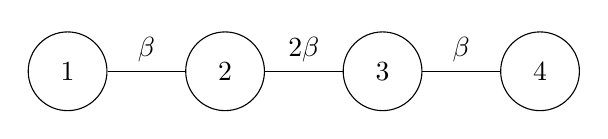
\begin{tikzpicture}
    % Draw nodes
    \node[circle, draw, fill=white, minimum size=1cm] (1) at (0,0) {1};
    \node[circle, draw, fill=white, minimum size=1cm] (2) at (2,0) {2};
    \node[circle, draw, fill=white, minimum size=1cm] (3) at (4,0) {3};
    \node[circle, draw, fill=white, minimum size=1cm] (4) at (6,0) {4};
    
    % Draw connections
    \draw[-] (1) -- (2) node[midway, above] {$\beta$};
    \draw[-] (2) -- (3) node[midway, above] {$2\beta$};
    \draw[-] (3) -- (4) node[midway, above] {$\beta$};
    
    % Labels
    \node[below] at (1) {};
    \node[below] at (2) {};
    \node[below] at (3) {};
    \node[below] at (4) {};
\end{tikzpicture}
\end{center}
\begin{center}
    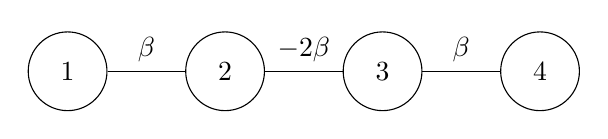
\begin{tikzpicture}
    % Draw nodes
    \node[circle, draw, fill=white, minimum size=1cm] (1) at (0,0) {1};
    \node[circle, draw, fill=white, minimum size=1cm] (2) at (2,0) {2};
    \node[circle, draw, fill=white, minimum size=1cm] (3) at (4,0) {3};
    \node[circle, draw, fill=white, minimum size=1cm] (4) at (6,0) {4};
    
    % Draw connections
    \draw[-] (1) -- (2) node[midway, above] {$\beta$};
    \draw[-] (2) -- (3) node[midway, above] {$-2\beta$};
    \draw[-] (3) -- (4) node[midway, above] {$\beta$};
    
    % Labels
    \node[below] at (1) {};
    \node[below] at (2) {};
    \node[below] at (3) {};
    \node[below] at (4) {};
\end{tikzpicture}
\end{center}
It was verified that in the configurations above, PST is possible from \textbf{node 1 and to node 3}. However,
\begin{equation}
    t=t'\neq\frac{\pi}{2\sqrt{2}\beta}
\end{equation}
Interestingly,
\begin{equation}
    t=t'=\frac{n\pi}{2\sqrt{2}\beta}
\end{equation}
where $n$ is a real positive integer.\\
However, another case demonstrated below, which is proven to exhibit PST from \textbf{node 1 to node 4}, cannot be found using the optimizer due to the fact that there are too many local minima in the loss value. The optimizer return no results most of the time.\\
\begin{center}
    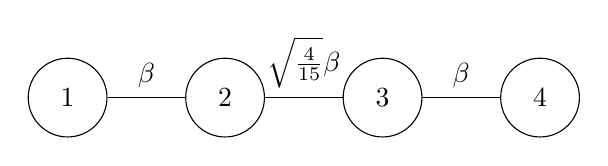
\begin{tikzpicture}
    % Draw nodes
    \node[circle, draw, fill=white, minimum size=1cm] (1) at (0,0) {1};
    \node[circle, draw, fill=white, minimum size=1cm] (2) at (2,0) {2};
    \node[circle, draw, fill=white, minimum size=1cm] (3) at (4,0) {3};
    \node[circle, draw, fill=white, minimum size=1cm] (4) at (6,0) {4};
    
    % Draw connections
    \draw[-] (1) -- (2) node[midway, above] {$\beta$};
    \draw[-] (2) -- (3) node[midway, above] {$\sqrt{\frac{4}{15}}\beta$};
    \draw[-] (3) -- (4) node[midway, above] {$\beta$};
    
    % Labels
    \node[below] at (1) {};
    \node[below] at (2) {};
    \node[below] at (3) {};
    \node[below] at (4) {};
\end{tikzpicture}
\end{center}
\begin{center}
    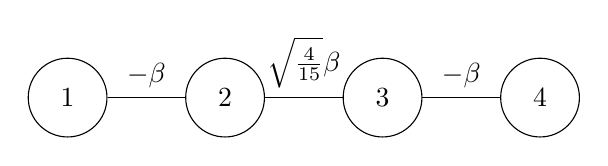
\begin{tikzpicture}
    % Draw nodes
    \node[circle, draw, fill=white, minimum size=1cm] (1) at (0,0) {1};
    \node[circle, draw, fill=white, minimum size=1cm] (2) at (2,0) {2};
    \node[circle, draw, fill=white, minimum size=1cm] (3) at (4,0) {3};
    \node[circle, draw, fill=white, minimum size=1cm] (4) at (6,0) {4};
    
    % Draw connections
    \draw[-] (1) -- (2) node[midway, above] {$-\beta$};
    \draw[-] (2) -- (3) node[midway, above] {$\sqrt{\frac{4}{15}}\beta$};
    \draw[-] (3) -- (4) node[midway, above] {$-\beta$};
    
    % Labels
    \node[below] at (1) {};
    \node[below] at (2) {};
    \node[below] at (3) {};
    \node[below] at (4) {};
\end{tikzpicture}
\end{center}
\begin{center}
    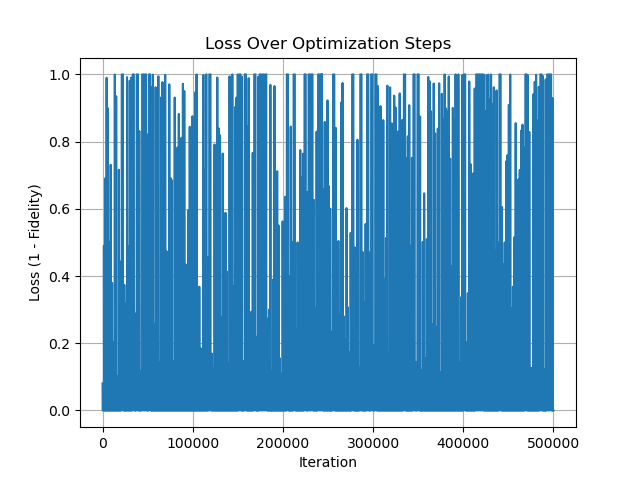
\includegraphics[width=0.7\textwidth]{loss.png}
\end{center}
I also found some solutions of PST from \textbf{node 1 to node 2} with the edge weights configurations below, but I have not attempted to work out the pattern yet.\\
\begin{center}
    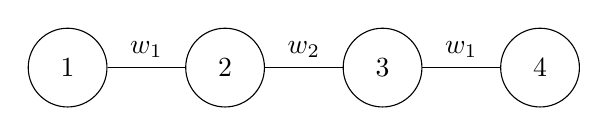
\begin{tikzpicture}
    % Draw nodes
    \node[circle, draw, fill=white, minimum size=1cm] (1) at (0,0) {1};
    \node[circle, draw, fill=white, minimum size=1cm] (2) at (2,0) {2};
    \node[circle, draw, fill=white, minimum size=1cm] (3) at (4,0) {3};
    \node[circle, draw, fill=white, minimum size=1cm] (4) at (6,0) {4};
    
    % Draw connections
    \draw[-] (1) -- (2) node[midway, above] {$w_1$};
    \draw[-] (2) -- (3) node[midway, above] {$w_2$};
    \draw[-] (3) -- (4) node[midway, above] {$w_1$};
    
    % Labels
    \node[below] at (1) {};
    \node[below] at (2) {};
    \node[below] at (3) {};
    \node[below] at (4) {};
\end{tikzpicture}
\end{center}
\begin{center}
    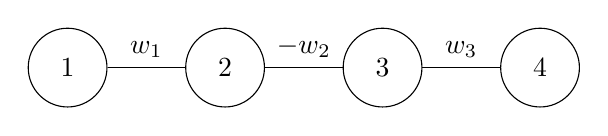
\begin{tikzpicture}
    % Draw nodes
    \node[circle, draw, fill=white, minimum size=1cm] (1) at (0,0) {1};
    \node[circle, draw, fill=white, minimum size=1cm] (2) at (2,0) {2};
    \node[circle, draw, fill=white, minimum size=1cm] (3) at (4,0) {3};
    \node[circle, draw, fill=white, minimum size=1cm] (4) at (6,0) {4};
    
    % Draw connections
    \draw[-] (1) -- (2) node[midway, above] {$w_1$};
    \draw[-] (2) -- (3) node[midway, above] {$-w_2$};
    \draw[-] (3) -- (4) node[midway, above] {$w_3$};
    
    % Labels
    \node[below] at (1) {};
    \node[below] at (2) {};
    \node[below] at (3) {};
    \node[below] at (4) {};
\end{tikzpicture}
\end{center}
One example is
\begin{verbatim}
Enter initial edge weights (space-separated, 3 values): 0.6626908221904778 -2.1850230509470592e-08 
0.6626908221904778
Enter final edge weights (space-separated, 3 values): 0.6626908221904778 2.1850230509470592e-08 
0.6626908221904778
Enter runtime before adjustment: 5.925826472411548
Enter runtime after adjustment: 5.925826472411548
    
Fidelity after full runtime: 1.000000000000000000000000000000
\end{verbatim}
This is the verification performed by the time evolution of quantum state code. The edge weight in the middle is pretty small, but it is still far from zero.\\
Here is another example:
\begin{verbatim}
Enter initial edge weights (space-separated, 3 values): 5.094830057973546 -6.170797557539656e-08 
5.094830057973546
Enter final edge weights (space-separated, 3 values): 5.094830057973546 6.170797557539656e-08 
5.094830057973546
Enter runtime before adjustment: 0.15415591008966015
Enter runtime after adjustment: 0.15415591008966015

Fidelity after full runtime: 1.000000000000000000000000000000
\end{verbatim}
This one is a bit weird, I wonder what leads to a fidelity slightly larger than 1:
\begin{verbatim}
Enter initial edge weights (space-separated, 3 values): 5.885431761530667 8.174164514679293e-07 
5.885431761530667
Enter final edge weights (space-separated, 3 values): 5.885431761530667 -8.174164514679293e-07 
5.885431761530667
Enter runtime before adjustment: 6.005152856
Enter runtime after adjustment: 6.005152856

Fidelity after full runtime: 1.000000000000007549516567451064
\end{verbatim}
\section{Questions}
\begin{enumerate}
    \item Discrepancies between the fidelities output between the validator and optimizer, which is likely caused by the accuracy differences between \texttt{tf.linalg.expm} and \texttt{scipy.linalg.expm}, where the latter is more accurate. Would it be beneficial to code the Adam's algorithm from scratch?
    \item Is $1$ actually $1$? Does a numerical fidelity of $1$ guarantee PST?
\end{enumerate}
\newpage
\section{P$_4$: Node 1 $\rightarrow$ Node 4 PST}
\subsection{0.999999999}
\begin{center}
    \begin{tabular}{||c c c||}
        \hline
        Initial Edge Weights&Final Edge Weights&$t=t'$\\
        \hline
        [1.0, 2.2677864162435357, 1.0]&[-1.0, 2.2677864162435357, -1.0]&2.081701141\\

        [1.0, 2.2677872585089562, 1.0]&[-1.0, 2.2677872585089562, -1.0]&2.0742356524309\\

        [1.0, -2.267787257589282, 1.0]&[-1.0, -2.267787257589282, -1.0]&2.074246026\\

        [1.0, -2.267786417033427, 1.0]&[-1.0, -2.267786417033427, -1.0]&2.08170109\\
        \hline
        [1.0, 0.5163978486429714, 1.0]&[-1.0, 0.5163978486429714, -1.0]&3.034013229\\
        
        [1.0, -0.5163973327358463, 1.0]&[-1.0, -0.5163973327358463, -1.0]&3.044563193\\

        [1.0, -0.5163978486459277, 1.0]&[-1.0, -0.5163978486459277, -1.0]&3.03401323\\
        \hline
        [1.0, 3.614820251255397, 1.0]&[-1.0, 3.614820251255397, -1.0]&3.04014415\\
        
        [1.0, -3.614785401654898, 1.0]&[-1.0, -3.614785401654898, -1.0]&3.03887772\\

        [1.0, -3.6147854023235837, 1.0]&[-1.0, -3.6147854023235837, -1.0]&3.038877381\\
        \hline
        [1.0, -4.587318653298133, 1.0]&[-1.0, -4.587318653298133, -1.0]&3.764012455\\
        
        [1.0, -4.587316594892395, 1.0]&[-1.0, -4.587316594892395, -1.0]&11.30253673\\

        [1.0, 4.587345143460048, 1.0]&[1.0, 4.587345143460048, 1.0]&3.767587833\\
        \hline
        [1.0, 5.388161262251575, 1.0]&[-1.0, 5.388161262251575, -1.0]&4.370490101\\

        [1.0, -5.388204386530768, 1.0]&[-1.0, -5.388204386530768, -1.0]&4.371473889\\
        \hline
        [1.0, -1.6012814463605203, 1.0]&[-1.0, -1.6012814463605203, -1.0]&4.909252167\\

        [1.0, -1.6012814463922922, 1.0]&[-1.0, -1.6012814463922922, -1.0]&4.909252043\\

        [1.0, -1.6012816295409682, 1.0]&[-1.0, -1.6012816295409682, -1.0]&4.9003682\\
        \hline
        [1.0, 6.084872739875749, 1.0]&[-1.0, 6.084872739875749, -1.0]&4.902530395\\

        [1.0, -6.084866925228957, 1.0]&[-1.0, -6.084866925228957, -1.0]&4.907089391\\

        [1.0, -6.084866943257897, 1.0]&[-1.0, -6.084866943257897, -1.0]&4.907089902\\
        \hline
        [1.0, -6.709793237392034, 1.0]&[-1.0, -6.709793237392034, -1.0]&5.382247619\\

        [1.0, -6.709793238127481, 1.0]&[-1.0, -6.709793238127481, -1.0]&5.382247074\\

        [1.0, -6.709785918264255, 1.0]&[-1.0, -6.709785918264255, -1.0]&5.386588214\\
        \hline
        [1.0, 0.809039874164738, 1.0]&[-1.0, 0.809039874164738, -1.0]&5.818418956\\

        [1.0, 0.8090386679103602, 1.0]&[-1.0, 0.8090386679103602, -1.0]&5.824430125\\

        [1.0, -0.8090398741444761, 1.0]&[-1.0, -0.8090398741444761, -1.0]&5.818420127\\
        \hline
        [1.0, -7.281369869968289, 1.0]&[-1.0, -7.281369869968289, -1.0]&5.822991142\\

        [1.0, -7.2813540562574275, 1.0]&[1.0, -7.2813540562574275, 1.0]&5.826753211\\

        [1.0, -7.2813541158043575, 1.0]&[-1.0, -7.2813541158043575, -1.0]&5.826752993\\
        \hline
        [1.0, -0.2519763555275555, 1.0]&[-1.0, -0.2519763555275555, -1.0]&6.222707537\\
        \hline
        [1.0, 7.81127097891731, 1.0]&[-1.0, 7.81127097891731, -1.0]&6.231891388\\

        [1.0, -7.811218900466319, 1.0]&[-1.0, -7.811218900466319, -1.0]&6.235755067\\

        [1.0, -7.811260571812177, 1.0]&[-1.0, -7.811260571812177, -1.0]&6.235917089\\
        \hline
        [1.0, -8.307465564796429, 1.0]&[-1.0, -8.307465564796429, -1.0]&6.619834791\\

        [1.0, -8.307477689698592, 1.0]&[-1.0, -8.307477689698592, -1.0]&6.615930995\\
        \hline
        [1.0, -8.775678756720122, 1.0]&[1.0, -8.775678756720122, 1.0]&6.982671079\\

        [1.0, -8.775692480914591, 1.0]&[-1.0, -8.775692480914591, -1.0]&6.978872379\\

        [1.0, -8.775692507093504, 1.0]&[-1.0, -8.775692507093504, -1.0]&6.978872542\\
        \hline
        [1.0, -2.7874927851808353, 1.0]&[-1.0, -2.7874927851808353, -1.0]&7.322339243\\

        [1.0, 2.7874923958166526, 1.0]&[-1.0, 2.7874923958166526, -1.0]&7.329073396\\
        \hline
        [1.0, -9.220175551480535, 1.0]&[-1.0, -9.220175551480535, -1.0]&7.323852643\\

        [1.0, -9.220160041813735, 1.0]&[-1.0, -9.220160041813735, -1.0]&7.327560054\\
        \hline
        [1.0, -9.644230191589418, 1.0]&[-1.0, -9.644230191589418, -1.0]&7.653361319\\
        \hline
    \end{tabular}
\end{center}
\begin{center}
    \begin{tabular}{||c c c||}
        \hline
        [1.0, -1.4363696430269532, 1.0]&[-1.0, -1.4363696430269532, -1.0]&7.659804294\\

        [1.0, -1.4363701167830498, 1.0]&[-1.0, -1.4363701167830498, -1.0]&7.650430304\\
        \hline
        [1.0, 10.050348592504676, 1.0]&[-1.0, 10.050348592504676, -1.0]&7.97269521\\
        \hline
        [1.0, -10.440748415133244, 1.0]&[-1.0, -10.440748415133244, -1.0]&8.272939815\\
        \hline
        [1.0, -3.227133528574531, 1.0]&[-1.0, -3.227133528574531, -1.0]&8.274232835\\

        [1.0, -3.2271369323243624, 1.0]&[-1.0, -3.2271369323243624, -1.0]&8.277812482\\
        \hline
        [1.0, 0.16724843366067466, 1.0]&[-1.0, 0.16724843366067466, -1.0]&9.378249982\\
        \hline
        [1.0, 3.9652583074360974, 1.0]&[-1.0, 3.9652583074360974, -1.0]&9.900671203\\
        
        [1.0, -3.96525830774512, 1.0]&[-1.0, -3.96525830774512, -1.0]&9.900670429\\
        \hline
        [1.0, -4.287482925652273, 1.0]&[-1.0, -4.287482925652273, -1.0]&10.6273849\\
        \hline 
    \end{tabular}
\end{center}
\subsection{0.999999999999}
\begin{center}
    \begin{tabular}{||c c c||}
        \hline
        Initial Edge Weights&Final Edge Weights&$t=t'$\\
        \hline
        [1.0, -2.267786840422201, 1.0]&[-1.0, -2.267786840422201, -1.0]&2.077304562\\

        [1.0, -2.267786840422201, 1.0]&[-1.0, -2.267786840422201, -1.0]&2.077304562\\

        [1.0, -2.267786840422201, 1.0]&[-1.0, -2.267786840422201, -1.0]&2.077304562\\
        \hline
        [1.0, 3.6147844511476226, 1.0]&[-1.0, 3.6147844511476226, -1.0]&3.042359822\\

        [1.0, 3.6147844511476226, 1.0]&[-1.0, 3.6147844511476226, -1.0]&3.042359822\\
        \hline
        [1.0, 4.587317100652229, 1.0]&[-1.0, 4.587317100652229, -1.0]&3.767103882\\
        \hline
        [1.0, 0.5163977791040121, 1.0]&[-1.0, 0.5163977791040121, -1.0]&3.043224841\\
        
        [1.0, 0.5163979082935659, 1.0]&[-1.0, 0.5163979082935659, -1.0]&3.041398719\\
        \hline
        [1.0, -5.388159048452486, 1.0]&[-1.0, -5.388159048452486, -1.0]&4.373342537\\

        [1.0, -5.388159073147655, 1.0]&[-1.0, -5.388159073147655, -1.0]&4.37248137\\
        \hline
        [1.0, 1.6012815385662786, 1.0]&[-1.0, 1.6012815385662786, -1.0]&4.904019911\\
        \hline
        [1.0, 0.8090399266807671, 1.0]&[-1.0, 0.8090399266807671, -1.0]&5.823707582\\

        [1.0, 0.8090398347456658, 1.0]&[-1.0, 0.8090398347456658, -1.0]&5.825780094\\

        [1.0, 0.8090398347456658, 1.0]&[-1.0, 0.8090398347456658, -1.0]&5.825780094\\
        \hline
        [1.0, 6.709789588696451, 1.0]&[-1.0, 6.709789588696451, -1.0]&5.384804545\\
        \hline
        [1.0, -0.2519763151128192, 1.0]&[-1.0, -0.2519763151128192, -1.0]&6.235895717\\
        \hline
    \end{tabular}
\end{center}
\subsection{0.999999999999999}
\begin{center}
    \begin{tabular}{||c c c||}
        \hline
        Initial Edge Weights&Final Edge Weights&$t=t'$\\
        \hline
        [1.0, -2.2677868380760757, 1.0]&[-1.0, -2.2677868380760757, -1.0]&2.077831382\\

        [1.0, -2.2677868380760757, 1.0]&[-1.0, -2.2677868380760757, -1.0]&2.077831382\\
        \hline
        [1.0, -7.281358514018219, 1.0]&[-1.0, -7.281358514018219, -1.0]&5.824775131\\
        \hline
        [1.0, 0.1672484025560938, 1.0]&[-1.0, 0.1672484025560938, -1.0]&9.392512825\\
        \hline
    \end{tabular}
\end{center}
\subsection{Exact Solutions}
\begin{center}
    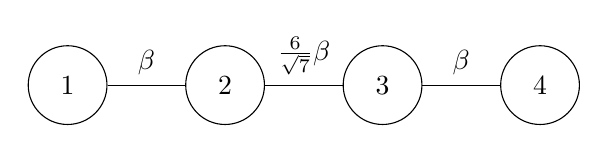
\begin{tikzpicture}
    % Draw nodes
    \node[circle, draw, fill=white, minimum size=1cm] (1) at (0,0) {1};
    \node[circle, draw, fill=white, minimum size=1cm] (2) at (2,0) {2};
    \node[circle, draw, fill=white, minimum size=1cm] (3) at (4,0) {3};
    \node[circle, draw, fill=white, minimum size=1cm] (4) at (6,0) {4};
    
    % Draw connections
    \draw[-] (1) -- (2) node[midway, above] {$\beta$};
    \draw[-] (2) -- (3) node[midway, above] {$\frac{6}{\sqrt{7}}\beta$};
    \draw[-] (3) -- (4) node[midway, above] {$\beta$};
    
    % Labels
    \node[below] at (1) {};
    \node[below] at (2) {};
    \node[below] at (3) {};
    \node[below] at (4) {};
\end{tikzpicture}
\end{center}
\begin{center}
    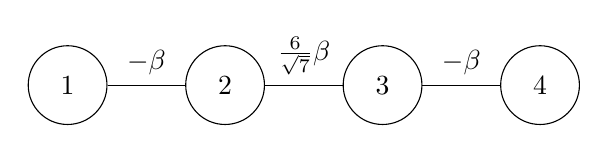
\begin{tikzpicture}
    % Draw nodes
    \node[circle, draw, fill=white, minimum size=1cm] (1) at (0,0) {1};
    \node[circle, draw, fill=white, minimum size=1cm] (2) at (2,0) {2};
    \node[circle, draw, fill=white, minimum size=1cm] (3) at (4,0) {3};
    \node[circle, draw, fill=white, minimum size=1cm] (4) at (6,0) {4};
    
    % Draw connections
    \draw[-] (1) -- (2) node[midway, above] {$-\beta$};
    \draw[-] (2) -- (3) node[midway, above] {$\frac{6}{\sqrt{7}}\beta$};
    \draw[-] (3) -- (4) node[midway, above] {$-\beta$};
    
    % Labels
    \node[below] at (1) {};
    \node[below] at (2) {};
    \node[below] at (3) {};
    \node[below] at (4) {};
\end{tikzpicture}
\end{center}
\begin{displaymath}
    t=t'=\frac{\sqrt{7}}{4\beta}\pi
\end{displaymath}
\noindent\rule{\textwidth}{0.5pt}
\begin{center}
    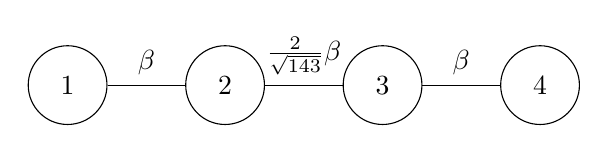
\begin{tikzpicture}
    % Draw nodes
    \node[circle, draw, fill=white, minimum size=1cm] (1) at (0,0) {1};
    \node[circle, draw, fill=white, minimum size=1cm] (2) at (2,0) {2};
    \node[circle, draw, fill=white, minimum size=1cm] (3) at (4,0) {3};
    \node[circle, draw, fill=white, minimum size=1cm] (4) at (6,0) {4};
    
    % Draw connections
    \draw[-] (1) -- (2) node[midway, above] {$\beta$};
    \draw[-] (2) -- (3) node[midway, above] {$\frac{2}{\sqrt{143}}\beta$};
    \draw[-] (3) -- (4) node[midway, above] {$\beta$};
    
    % Labels
    \node[below] at (1) {};
    \node[below] at (2) {};
    \node[below] at (3) {};
    \node[below] at (4) {};
\end{tikzpicture}
\end{center}
\begin{center}
    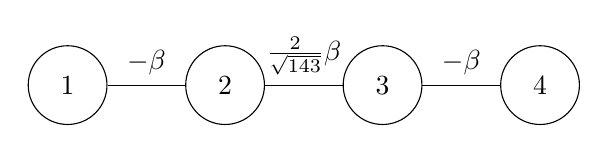
\begin{tikzpicture}
    % Draw nodes
    \node[circle, draw, fill=white, minimum size=1cm] (1) at (0,0) {1};
    \node[circle, draw, fill=white, minimum size=1cm] (2) at (2,0) {2};
    \node[circle, draw, fill=white, minimum size=1cm] (3) at (4,0) {3};
    \node[circle, draw, fill=white, minimum size=1cm] (4) at (6,0) {4};
    
    % Draw connections
    \draw[-] (1) -- (2) node[midway, above] {$-\beta$};
    \draw[-] (2) -- (3) node[midway, above] {$\frac{2}{\sqrt{143}}\beta$};
    \draw[-] (3) -- (4) node[midway, above] {$-\beta$};
    
    % Labels
    \node[below] at (1) {};
    \node[below] at (2) {};
    \node[below] at (3) {};
    \node[below] at (4) {};
\end{tikzpicture}
\end{center}
\begin{displaymath}
    t=t'=\frac{\sqrt{143}}{4\beta}\pi
\end{displaymath}
\noindent\rule{\textwidth}{0.5pt}
\begin{center}
    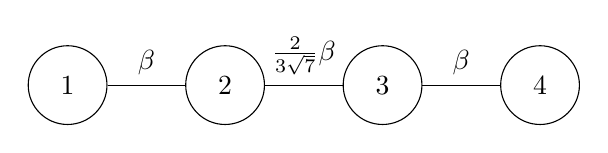
\begin{tikzpicture}
    % Draw nodes
    \node[circle, draw, fill=white, minimum size=1cm] (1) at (0,0) {1};
    \node[circle, draw, fill=white, minimum size=1cm] (2) at (2,0) {2};
    \node[circle, draw, fill=white, minimum size=1cm] (3) at (4,0) {3};
    \node[circle, draw, fill=white, minimum size=1cm] (4) at (6,0) {4};
    
    % Draw connections
    \draw[-] (1) -- (2) node[midway, above] {$\beta$};
    \draw[-] (2) -- (3) node[midway, above] {$\frac{2}{3\sqrt{7}}\beta$};
    \draw[-] (3) -- (4) node[midway, above] {$\beta$};
    
    % Labels
    \node[below] at (1) {};
    \node[below] at (2) {};
    \node[below] at (3) {};
    \node[below] at (4) {};
\end{tikzpicture}
\end{center}
\begin{center}
    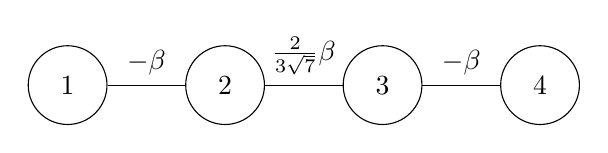
\begin{tikzpicture}
    % Draw nodes
    \node[circle, draw, fill=white, minimum size=1cm] (1) at (0,0) {1};
    \node[circle, draw, fill=white, minimum size=1cm] (2) at (2,0) {2};
    \node[circle, draw, fill=white, minimum size=1cm] (3) at (4,0) {3};
    \node[circle, draw, fill=white, minimum size=1cm] (4) at (6,0) {4};
    
    % Draw connections
    \draw[-] (1) -- (2) node[midway, above] {$-\beta$};
    \draw[-] (2) -- (3) node[midway, above] {$\frac{2}{3\sqrt{7}}\beta$};
    \draw[-] (3) -- (4) node[midway, above] {$-\beta$};
    
    % Labels
    \node[below] at (1) {};
    \node[below] at (2) {};
    \node[below] at (3) {};
    \node[below] at (4) {};
\end{tikzpicture}
\end{center}
\begin{displaymath}
    t=t'=\frac{3\sqrt{7}}{4\beta}\pi
\end{displaymath}
\noindent\rule{\textwidth}{0.5pt}
\begin{center}
    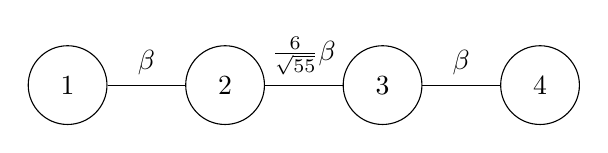
\begin{tikzpicture}
    % Draw nodes
    \node[circle, draw, fill=white, minimum size=1cm] (1) at (0,0) {1};
    \node[circle, draw, fill=white, minimum size=1cm] (2) at (2,0) {2};
    \node[circle, draw, fill=white, minimum size=1cm] (3) at (4,0) {3};
    \node[circle, draw, fill=white, minimum size=1cm] (4) at (6,0) {4};
    
    % Draw connections
    \draw[-] (1) -- (2) node[midway, above] {$\beta$};
    \draw[-] (2) -- (3) node[midway, above] {$\frac{6}{\sqrt{55}}\beta$};
    \draw[-] (3) -- (4) node[midway, above] {$\beta$};
    
    % Labels
    \node[below] at (1) {};
    \node[below] at (2) {};
    \node[below] at (3) {};
    \node[below] at (4) {};
\end{tikzpicture}
\end{center}
\begin{center}
    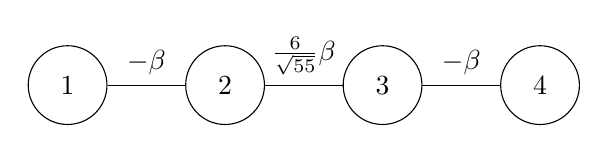
\begin{tikzpicture}
    % Draw nodes
    \node[circle, draw, fill=white, minimum size=1cm] (1) at (0,0) {1};
    \node[circle, draw, fill=white, minimum size=1cm] (2) at (2,0) {2};
    \node[circle, draw, fill=white, minimum size=1cm] (3) at (4,0) {3};
    \node[circle, draw, fill=white, minimum size=1cm] (4) at (6,0) {4};
    
    % Draw connections
    \draw[-] (1) -- (2) node[midway, above] {$-\beta$};
    \draw[-] (2) -- (3) node[midway, above] {$\frac{6}{\sqrt{55}}\beta$};
    \draw[-] (3) -- (4) node[midway, above] {$-\beta$};
    
    % Labels
    \node[below] at (1) {};
    \node[below] at (2) {};
    \node[below] at (3) {};
    \node[below] at (4) {};
\end{tikzpicture}
\end{center}
\begin{displaymath}
    t=t'=\frac{\sqrt{55}}{4\beta}\pi
\end{displaymath}
\noindent\rule{\textwidth}{0.5pt}
\begin{center}
    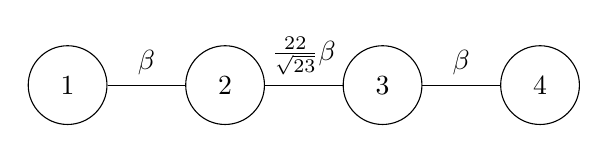
\begin{tikzpicture}
    % Draw nodes
    \node[circle, draw, fill=white, minimum size=1cm] (1) at (0,0) {1};
    \node[circle, draw, fill=white, minimum size=1cm] (2) at (2,0) {2};
    \node[circle, draw, fill=white, minimum size=1cm] (3) at (4,0) {3};
    \node[circle, draw, fill=white, minimum size=1cm] (4) at (6,0) {4};
    
    % Draw connections
    \draw[-] (1) -- (2) node[midway, above] {$\beta$};
    \draw[-] (2) -- (3) node[midway, above] {$\frac{22}{\sqrt{23}}\beta$};
    \draw[-] (3) -- (4) node[midway, above] {$\beta$};
    
    % Labels
    \node[below] at (1) {};
    \node[below] at (2) {};
    \node[below] at (3) {};
    \node[below] at (4) {};
\end{tikzpicture}
\end{center}
\begin{center}
    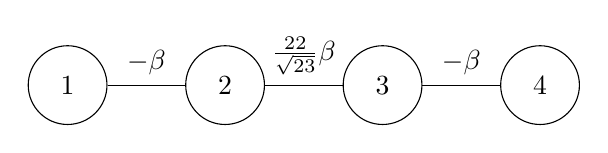
\begin{tikzpicture}
    % Draw nodes
    \node[circle, draw, fill=white, minimum size=1cm] (1) at (0,0) {1};
    \node[circle, draw, fill=white, minimum size=1cm] (2) at (2,0) {2};
    \node[circle, draw, fill=white, minimum size=1cm] (3) at (4,0) {3};
    \node[circle, draw, fill=white, minimum size=1cm] (4) at (6,0) {4};
    
    % Draw connections
    \draw[-] (1) -- (2) node[midway, above] {$-\beta$};
    \draw[-] (2) -- (3) node[midway, above] {$\frac{22}{\sqrt{23}}\beta$};
    \draw[-] (3) -- (4) node[midway, above] {$-\beta$};
    
    % Labels
    \node[below] at (1) {};
    \node[below] at (2) {};
    \node[below] at (3) {};
    \node[below] at (4) {};
\end{tikzpicture}
\end{center}
\begin{displaymath}
    t=t'=\frac{\sqrt{23}}{4\beta}\pi
\end{displaymath}
\noindent\rule{\textwidth}{0.5pt}
\newpage
\begin{center}
    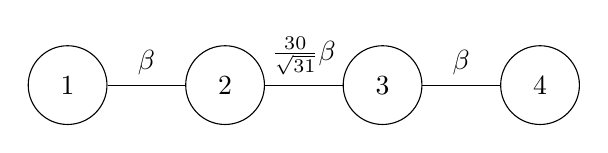
\begin{tikzpicture}
    % Draw nodes
    \node[circle, draw, fill=white, minimum size=1cm] (1) at (0,0) {1};
    \node[circle, draw, fill=white, minimum size=1cm] (2) at (2,0) {2};
    \node[circle, draw, fill=white, minimum size=1cm] (3) at (4,0) {3};
    \node[circle, draw, fill=white, minimum size=1cm] (4) at (6,0) {4};
    
    % Draw connections
    \draw[-] (1) -- (2) node[midway, above] {$\beta$};
    \draw[-] (2) -- (3) node[midway, above] {$\frac{30}{\sqrt{31}}\beta$};
    \draw[-] (3) -- (4) node[midway, above] {$\beta$};
    
    % Labels
    \node[below] at (1) {};
    \node[below] at (2) {};
    \node[below] at (3) {};
    \node[below] at (4) {};
\end{tikzpicture}
\end{center}
\begin{center}
    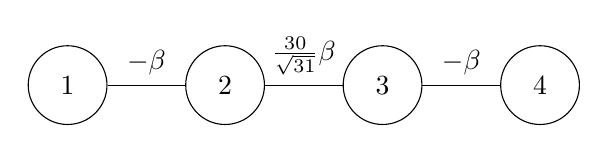
\begin{tikzpicture}
    % Draw nodes
    \node[circle, draw, fill=white, minimum size=1cm] (1) at (0,0) {1};
    \node[circle, draw, fill=white, minimum size=1cm] (2) at (2,0) {2};
    \node[circle, draw, fill=white, minimum size=1cm] (3) at (4,0) {3};
    \node[circle, draw, fill=white, minimum size=1cm] (4) at (6,0) {4};
    
    % Draw connections
    \draw[-] (1) -- (2) node[midway, above] {$-\beta$};
    \draw[-] (2) -- (3) node[midway, above] {$\frac{30}{\sqrt{31}}\beta$};
    \draw[-] (3) -- (4) node[midway, above] {$-\beta$};
    
    % Labels
    \node[below] at (1) {};
    \node[below] at (2) {};
    \node[below] at (3) {};
    \node[below] at (4) {};
\end{tikzpicture}
\end{center}
\begin{displaymath}
    t=t'=\frac{\sqrt{31}}{4\beta}\pi
\end{displaymath}
\noindent\rule{\textwidth}{0.5pt}
\begin{center}
    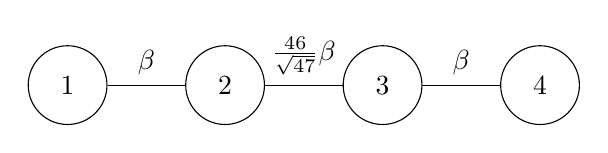
\begin{tikzpicture}
    % Draw nodes
    \node[circle, draw, fill=white, minimum size=1cm] (1) at (0,0) {1};
    \node[circle, draw, fill=white, minimum size=1cm] (2) at (2,0) {2};
    \node[circle, draw, fill=white, minimum size=1cm] (3) at (4,0) {3};
    \node[circle, draw, fill=white, minimum size=1cm] (4) at (6,0) {4};
    
    % Draw connections
    \draw[-] (1) -- (2) node[midway, above] {$\beta$};
    \draw[-] (2) -- (3) node[midway, above] {$\frac{46}{\sqrt{47}}\beta$};
    \draw[-] (3) -- (4) node[midway, above] {$\beta$};
    
    % Labels
    \node[below] at (1) {};
    \node[below] at (2) {};
    \node[below] at (3) {};
    \node[below] at (4) {};
\end{tikzpicture}
\end{center}
\begin{center}
    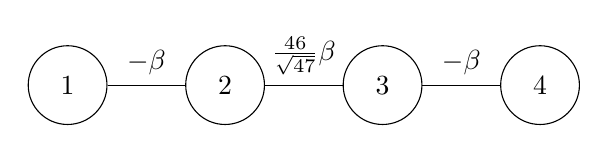
\begin{tikzpicture}
    % Draw nodes
    \node[circle, draw, fill=white, minimum size=1cm] (1) at (0,0) {1};
    \node[circle, draw, fill=white, minimum size=1cm] (2) at (2,0) {2};
    \node[circle, draw, fill=white, minimum size=1cm] (3) at (4,0) {3};
    \node[circle, draw, fill=white, minimum size=1cm] (4) at (6,0) {4};
    
    % Draw connections
    \draw[-] (1) -- (2) node[midway, above] {$-\beta$};
    \draw[-] (2) -- (3) node[midway, above] {$\frac{46}{\sqrt{47}}\beta$};
    \draw[-] (3) -- (4) node[midway, above] {$-\beta$};
    
    % Labels
    \node[below] at (1) {};
    \node[below] at (2) {};
    \node[below] at (3) {};
    \node[below] at (4) {};
\end{tikzpicture}
\end{center}
\begin{displaymath}
    t=t'=\frac{\sqrt{47}}{4\beta}\pi
\end{displaymath}
\noindent\rule{\textwidth}{0.5pt}
\begin{center}
    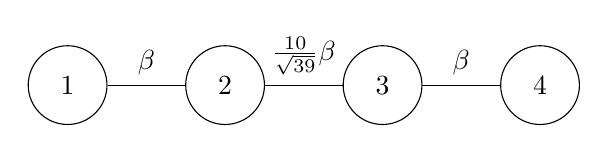
\begin{tikzpicture}
    % Draw nodes
    \node[circle, draw, fill=white, minimum size=1cm] (1) at (0,0) {1};
    \node[circle, draw, fill=white, minimum size=1cm] (2) at (2,0) {2};
    \node[circle, draw, fill=white, minimum size=1cm] (3) at (4,0) {3};
    \node[circle, draw, fill=white, minimum size=1cm] (4) at (6,0) {4};
    
    % Draw connections
    \draw[-] (1) -- (2) node[midway, above] {$\beta$};
    \draw[-] (2) -- (3) node[midway, above] {$\frac{10}{\sqrt{39}}\beta$};
    \draw[-] (3) -- (4) node[midway, above] {$\beta$};
    
    % Labels
    \node[below] at (1) {};
    \node[below] at (2) {};
    \node[below] at (3) {};
    \node[below] at (4) {};
\end{tikzpicture}
\end{center}
\begin{center}
    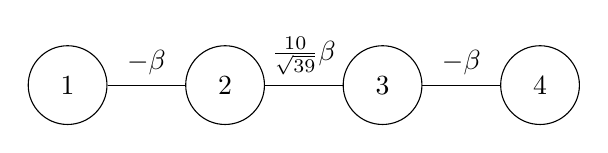
\begin{tikzpicture}
    % Draw nodes
    \node[circle, draw, fill=white, minimum size=1cm] (1) at (0,0) {1};
    \node[circle, draw, fill=white, minimum size=1cm] (2) at (2,0) {2};
    \node[circle, draw, fill=white, minimum size=1cm] (3) at (4,0) {3};
    \node[circle, draw, fill=white, minimum size=1cm] (4) at (6,0) {4};
    
    % Draw connections
    \draw[-] (1) -- (2) node[midway, above] {$-\beta$};
    \draw[-] (2) -- (3) node[midway, above] {$\frac{10}{\sqrt{39}}\beta$};
    \draw[-] (3) -- (4) node[midway, above] {$-\beta$};
    
    % Labels
    \node[below] at (1) {};
    \node[below] at (2) {};
    \node[below] at (3) {};
    \node[below] at (4) {};
\end{tikzpicture}
\end{center}
\begin{displaymath}
    t=t'=\frac{\sqrt{39}}{4\beta}\pi
\end{displaymath}
\noindent\rule{\textwidth}{0.5pt}
\subsection{Possible Relations}
\begin{center}
    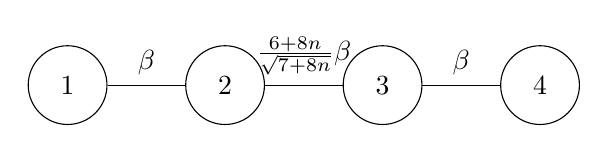
\begin{tikzpicture}
    % Draw nodes
    \node[circle, draw, fill=white, minimum size=1cm] (1) at (0,0) {1};
    \node[circle, draw, fill=white, minimum size=1cm] (2) at (2,0) {2};
    \node[circle, draw, fill=white, minimum size=1cm] (3) at (4,0) {3};
    \node[circle, draw, fill=white, minimum size=1cm] (4) at (6,0) {4};
    
    % Draw connections
    \draw[-] (1) -- (2) node[midway, above] {$\beta$};
    \draw[-] (2) -- (3) node[midway, above] {$\frac{6+8n}{\sqrt{7+8n}}\beta$};
    \draw[-] (3) -- (4) node[midway, above] {$\beta$};
    
    % Labels
    \node[below] at (1) {};
    \node[below] at (2) {};
    \node[below] at (3) {};
    \node[below] at (4) {};
\end{tikzpicture}
\end{center}
\begin{center}
    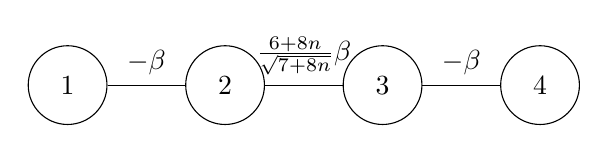
\begin{tikzpicture}
    % Draw nodes
    \node[circle, draw, fill=white, minimum size=1cm] (1) at (0,0) {1};
    \node[circle, draw, fill=white, minimum size=1cm] (2) at (2,0) {2};
    \node[circle, draw, fill=white, minimum size=1cm] (3) at (4,0) {3};
    \node[circle, draw, fill=white, minimum size=1cm] (4) at (6,0) {4};
    
    % Draw connections
    \draw[-] (1) -- (2) node[midway, above] {$-\beta$};
    \draw[-] (2) -- (3) node[midway, above] {$\frac{6+8n}{\sqrt{7+8n}}\beta$};
    \draw[-] (3) -- (4) node[midway, above] {$-\beta$};
    
    % Labels
    \node[below] at (1) {};
    \node[below] at (2) {};
    \node[below] at (3) {};
    \node[below] at (4) {};
\end{tikzpicture}
\end{center}
\begin{displaymath}
    t=t'=\frac{\sqrt{7+8n}}{4\beta}\pi,\quad(n\in\mathbb{Z})
\end{displaymath}
\noindent\rule{\textwidth}{0.5pt}
\newpage
\subsection{$t=t'$ and $t\neq t'$}
\begin{center}
    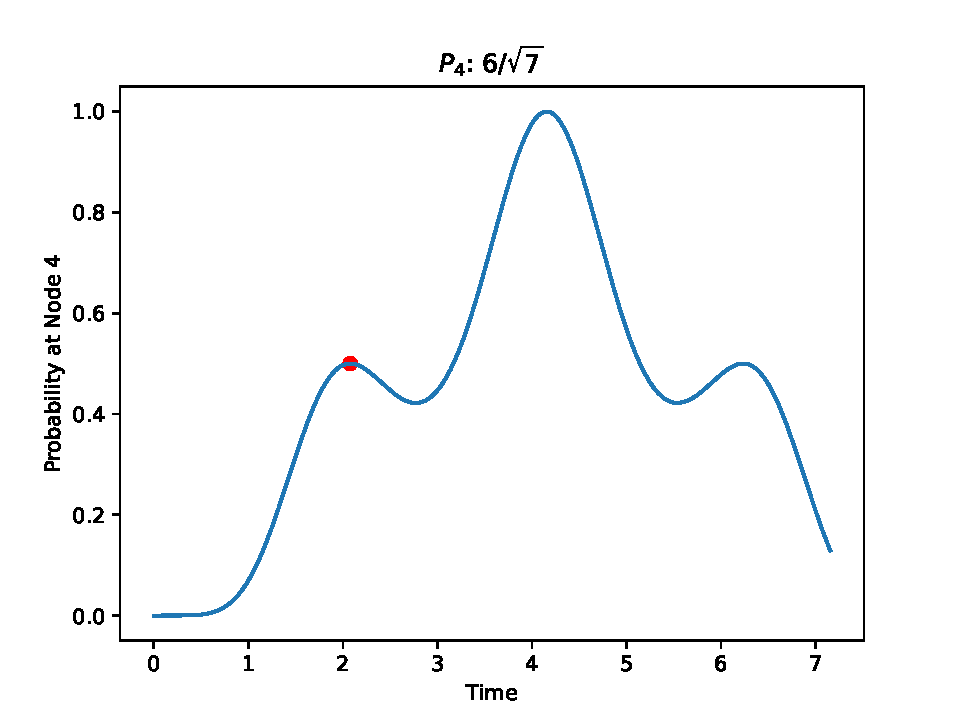
\includegraphics[width=0.7\textwidth]{different time 1.pdf}
\end{center}
\begin{displaymath}
    t=t'=\frac{\sqrt{7}}{4}\pi
\end{displaymath}
\begin{center}
    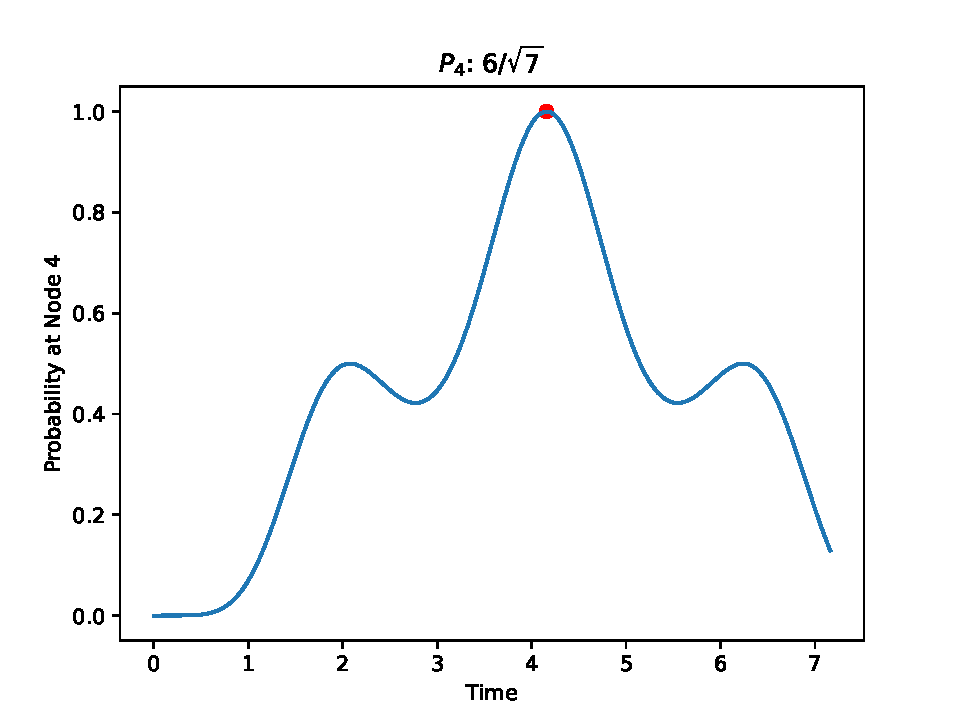
\includegraphics[width=0.7\textwidth]{different time 2.pdf}
\end{center}
\begin{displaymath}
    t=4.157761123,\quad t'=0.001787291
\end{displaymath}
\begin{center}
    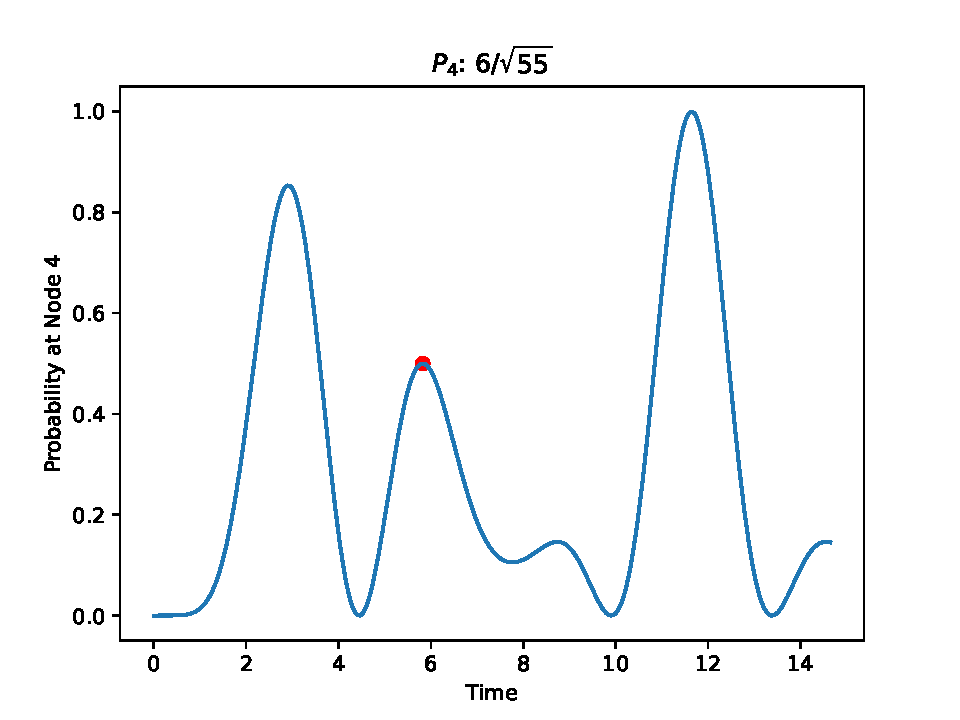
\includegraphics[width=0.7\textwidth]{different time 3.pdf}
\end{center}
\begin{displaymath}
    t=t'=\frac{\sqrt{55}}{4}\pi
\end{displaymath}
\begin{center}
    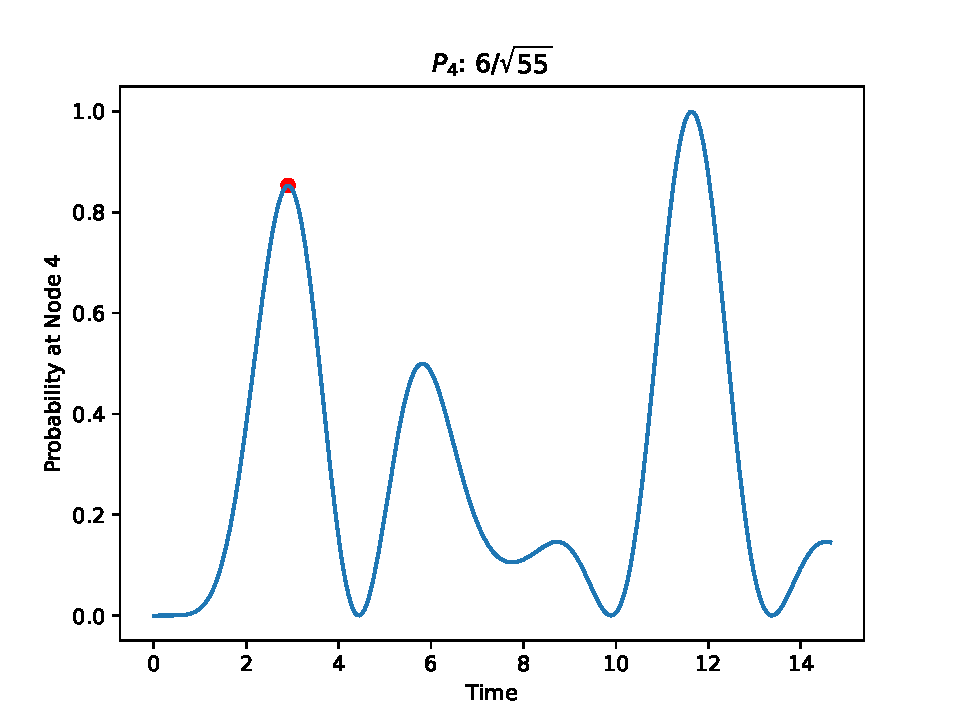
\includegraphics[width=0.7\textwidth]{different time 4.pdf}
\end{center}
\begin{displaymath}
    t=2.906083132,\quad t'=8.730751769
\end{displaymath}
\begin{center}
    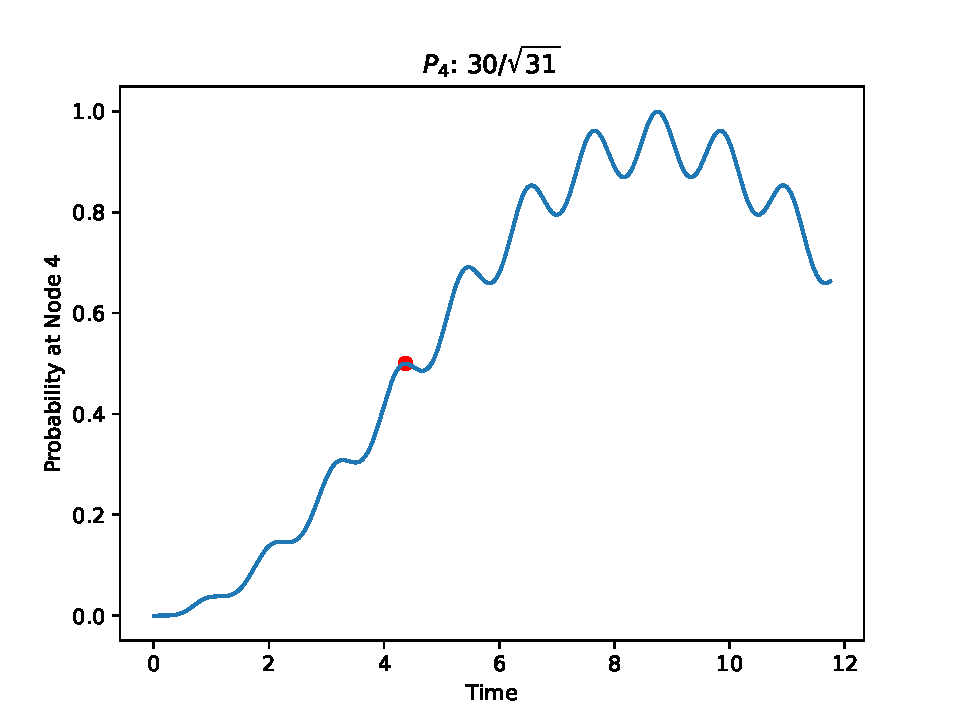
\includegraphics[width=0.7\textwidth]{different time 5.pdf}
\end{center}
\begin{displaymath}
    t=t'=\frac{\sqrt{31}}{4}\pi
\end{displaymath}
\begin{center}
    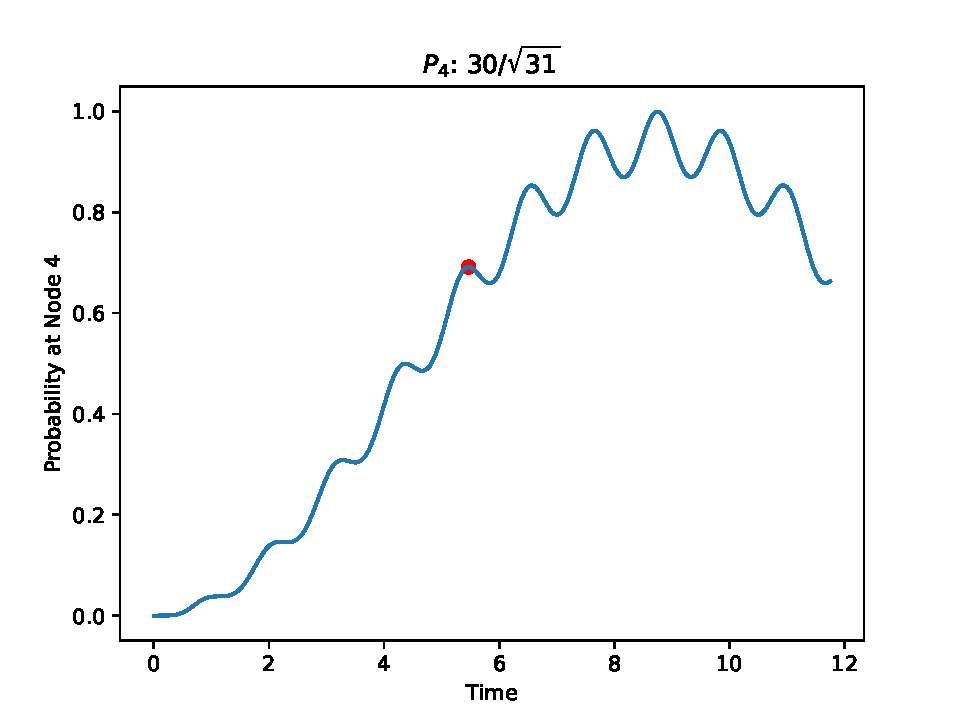
\includegraphics[width=0.7\textwidth]{different time 6.pdf}
\end{center}
\begin{displaymath}
    t=5.468562326,\quad t'=3.282105682
\end{displaymath}
\begin{center}
    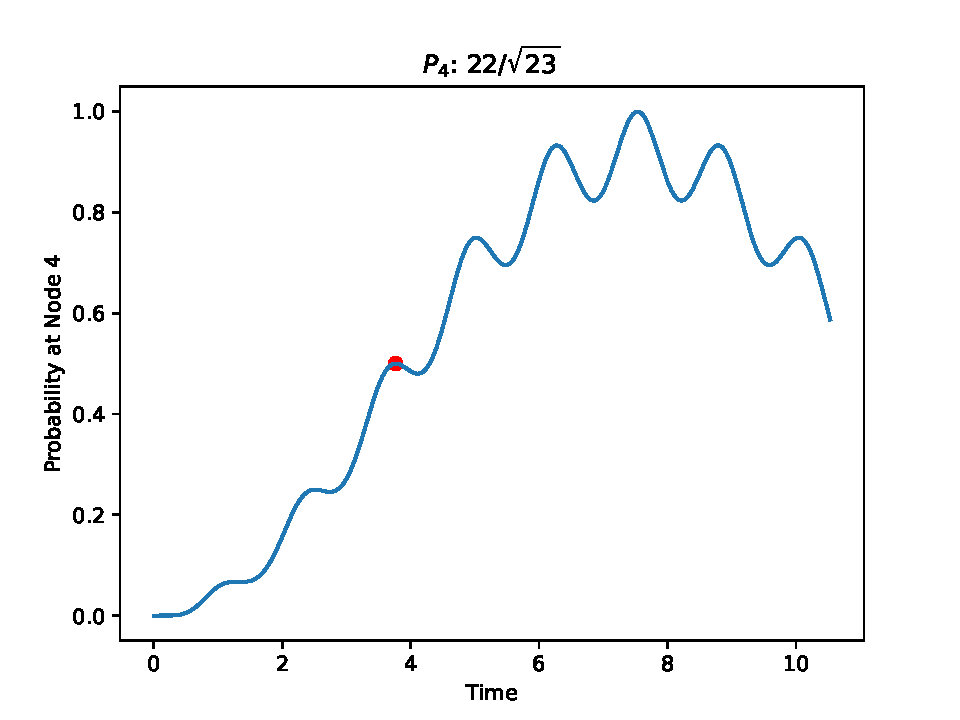
\includegraphics[width=0.7\textwidth]{different time 7.pdf}
\end{center}
\begin{displaymath}
    t=t'=\frac{\sqrt{23}}{4}\pi
\end{displaymath}
\begin{center}
    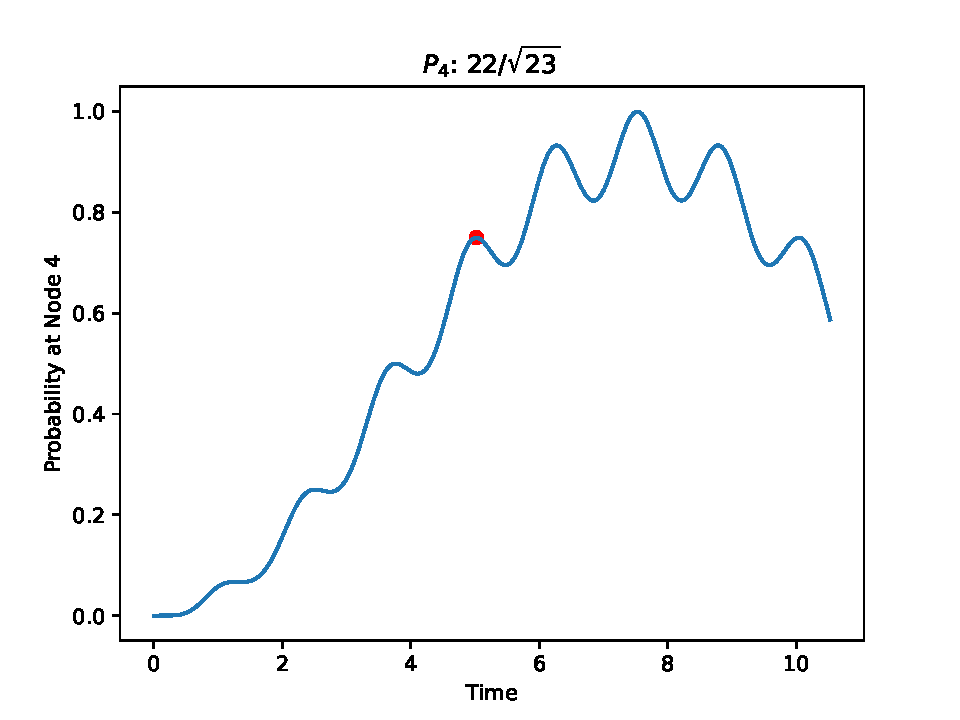
\includegraphics[width=0.7\textwidth]{different time 8.pdf}
\end{center}
\begin{displaymath}
    t=5.019558545,\quad t'=2.50846772
\end{displaymath}
\subsection{The Golden Rule?}
\begin{center}
    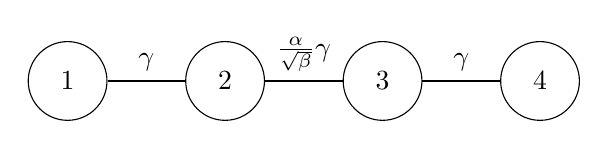
\begin{tikzpicture}
        % Draw nodes
        \node[circle, draw, fill=white, minimum size=1cm] (1) at (0,0) {1};
        \node[circle, draw, fill=white, minimum size=1cm] (2) at (2,0) {2};
        \node[circle, draw, fill=white, minimum size=1cm] (3) at (4,0) {3};
        \node[circle, draw, fill=white, minimum size=1cm] (4) at (6,0) {4};
        
        % Draw connections
        \draw[-] (1) -- (2) node[midway, above] {$\gamma$};
        \draw[-] (2) -- (3) node[midway, above] {$\frac{\alpha}{\sqrt{\beta}} \gamma$};
        \draw[-] (3) -- (4) node[midway, above] {$\gamma$};
    \end{tikzpicture}
\end{center}
\begin{center}
    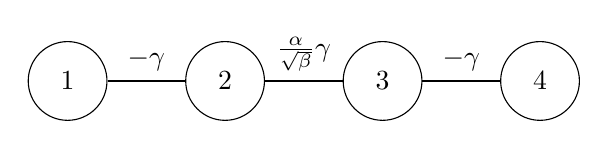
\begin{tikzpicture}
        % Draw nodes
        \node[circle, draw, fill=white, minimum size=1cm] (1) at (0,0) {1};
        \node[circle, draw, fill=white, minimum size=1cm] (2) at (2,0) {2};
        \node[circle, draw, fill=white, minimum size=1cm] (3) at (4,0) {3};
        \node[circle, draw, fill=white, minimum size=1cm] (4) at (6,0) {4};
        
        % Draw connections
        \draw[-] (1) -- (2) node[midway, above] {$-\gamma$};
        \draw[-] (2) -- (3) node[midway, above] {$\frac{\alpha}{\sqrt{\beta}} \gamma$};
        \draw[-] (3) -- (4) node[midway, above] {$-\gamma$};
    \end{tikzpicture}
\end{center}
\begin{align*}
    \beta &= 7 + 8n = (5+p)(3 - p + 8m), \\
    \alpha &= 2 + 2p - 8m, \\
    &\text{where} \quad
    \begin{cases}
        n = 0,1,2,\dots, \\
        m = 0,1,2,\dots,n.
    \end{cases}
\end{align*}
If $p\in\mathbb{Z}$ and $\nicefrac{\alpha}{\sqrt{\beta}}$ is in its simplest form $\nicefrac{\alpha'}{\sqrt{\beta'}}$ where $\alpha',\beta'\in\mathbb{Z}$, then the shortest time needed for two-step PST is
\begin{displaymath}
    t = t' = \frac{\sqrt{\beta'} \pi}{4\gamma}.
\end{displaymath}
The shortest time needed for one-step PST is
\begin{displaymath}
    t = t' = \frac{\sqrt{\beta'} \pi}{2\gamma}.
\end{displaymath}
\newpage
\section{C$_3$ Node 1 $\rightarrow$ Node 2 PST}
\begin{center}
    \begin{tikzpicture}
    % Draw nodes
    \node[circle, draw, fill=white, minimum size=1cm] (1) at (0,1.5) {1};
    \node[circle, draw, fill=white, minimum size=1cm] (2) at (2.6,-1.5) {2};
    \node[circle, draw, fill=white, minimum size=1cm] (3) at (-2.6,-1.5) {3};
    
    % Draw connections
    \draw[-] (1) -- (2) node[midway, right] {$1$};
    \draw[-] (2) -- (3) node[midway, below] {$\beta$};
    \draw[-] (3) -- (1) node[midway, left] {$\beta$};
    
    % Labels
    \node[below] at (1) {};
    \node[below] at (2) {};
    \node[below] at (3) {};
\end{tikzpicture}
\end{center}
\begin{center}
    \begin{tikzpicture}
    % Draw nodes
    \node[circle, draw, fill=white, minimum size=1cm] (1) at (0,1.5) {1};
    \node[circle, draw, fill=white, minimum size=1cm] (2) at (2.6,-1.5) {2};
    \node[circle, draw, fill=white, minimum size=1cm] (3) at (-2.6,-1.5) {3};
    
    % Draw connections
    \draw[-] (1) -- (2) node[midway, right] {$1$};
    \draw[-] (2) -- (3) node[midway, below] {$\beta$};
    \draw[-] (3) -- (1) node[midway, left] {$-\beta$};
    
    % Labels
    \node[below] at (1) {};
    \node[below] at (2) {};
    \node[below] at (3) {};
\end{tikzpicture}
\end{center}
\subsection{Is Two-Step Necessary?}
\begin{center}
    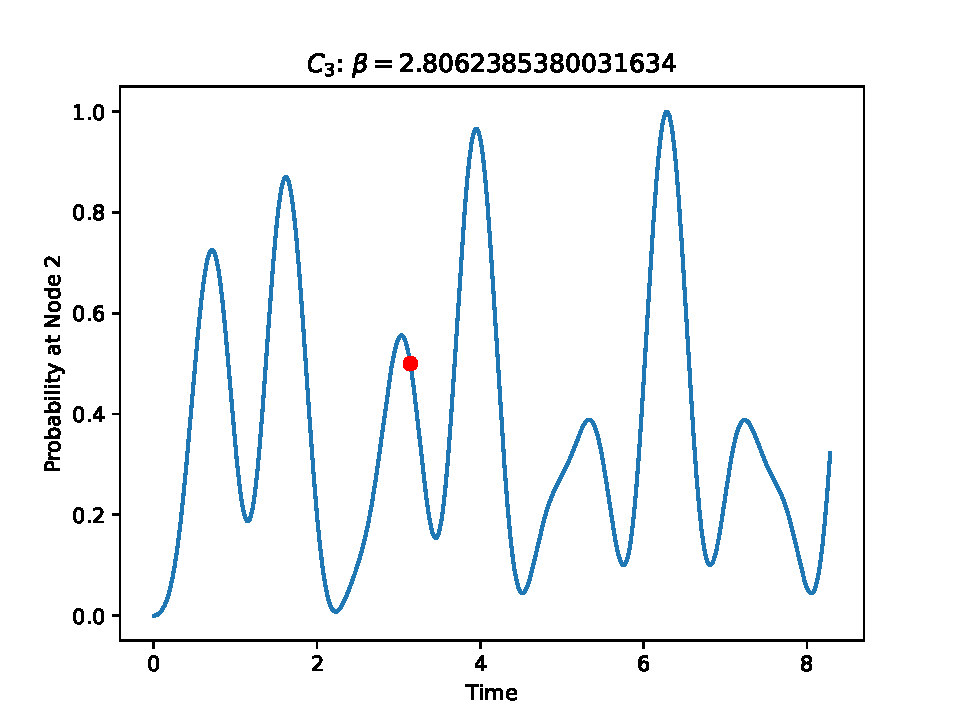
\includegraphics[width=0.7\textwidth]{c_3 (1).pdf}
\end{center}
\begin{displaymath}
    t=t'=\pi
\end{displaymath}
\begin{center}
    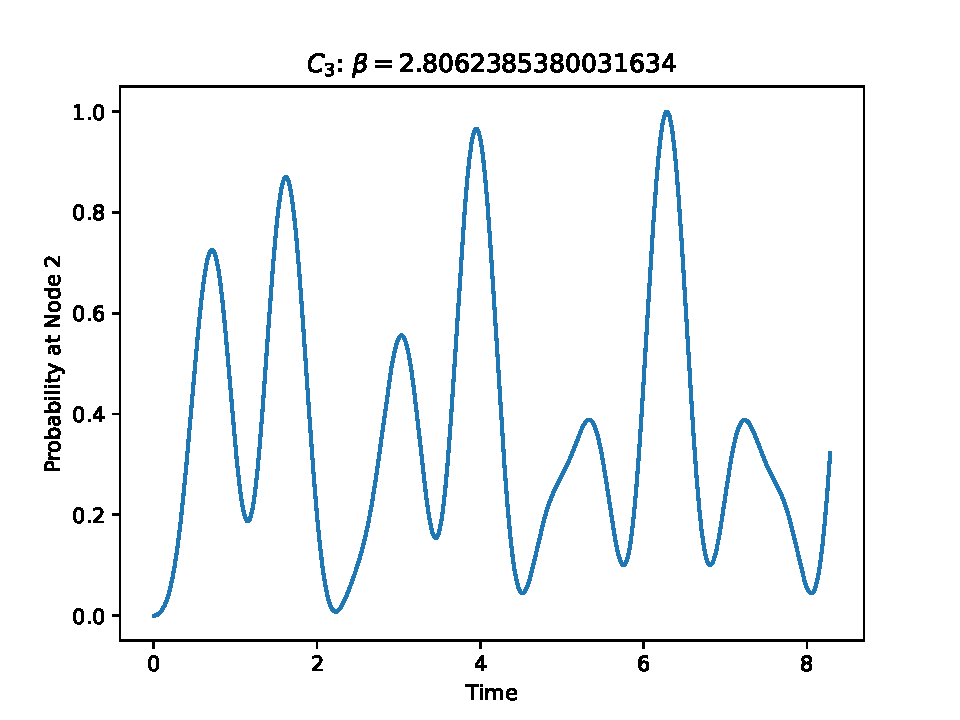
\includegraphics[width=0.7\textwidth]{c_3 (2).pdf}
\end{center}
\begin{displaymath}
    t=2\pi
\end{displaymath}
\begin{center}
    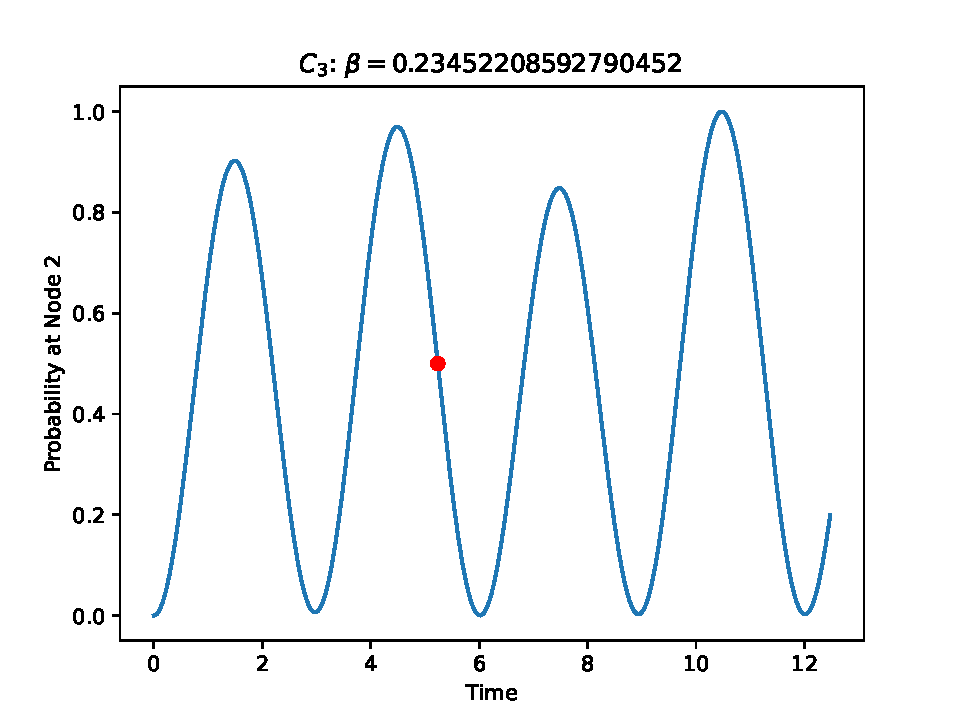
\includegraphics[width=0.7\textwidth]{c_3 (3).pdf}
\end{center}
\begin{displaymath}
    t=t'=\frac{5\pi}{3}
\end{displaymath}
\begin{center}
    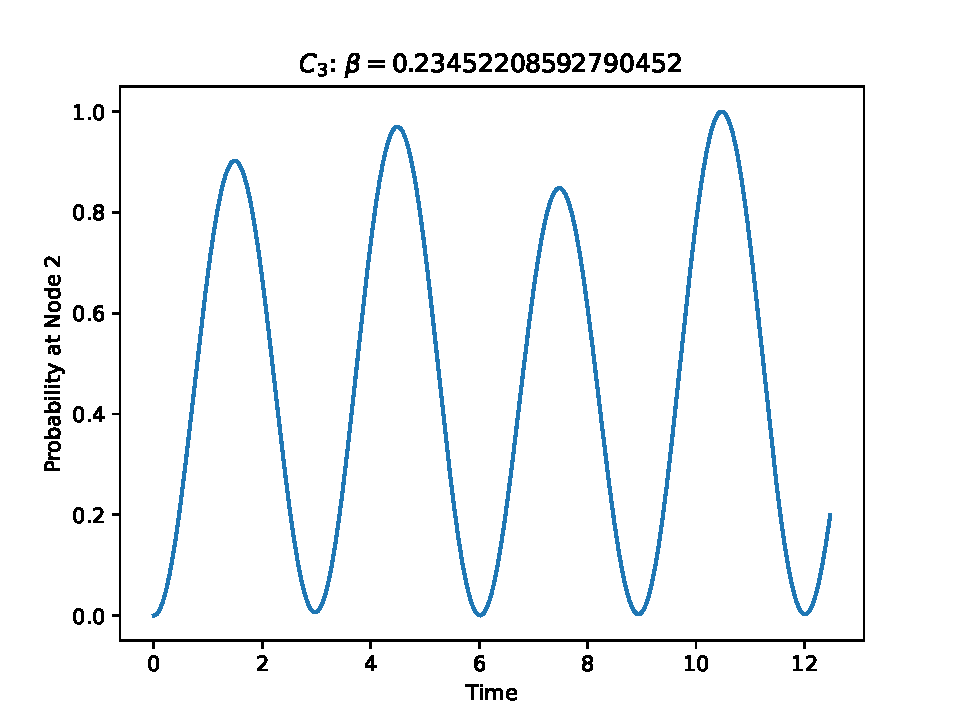
\includegraphics[width=0.7\textwidth]{c_3 (4).pdf}
\end{center}
\begin{displaymath}
    t=\frac{10\pi}{3}
\end{displaymath}
\begin{center}
    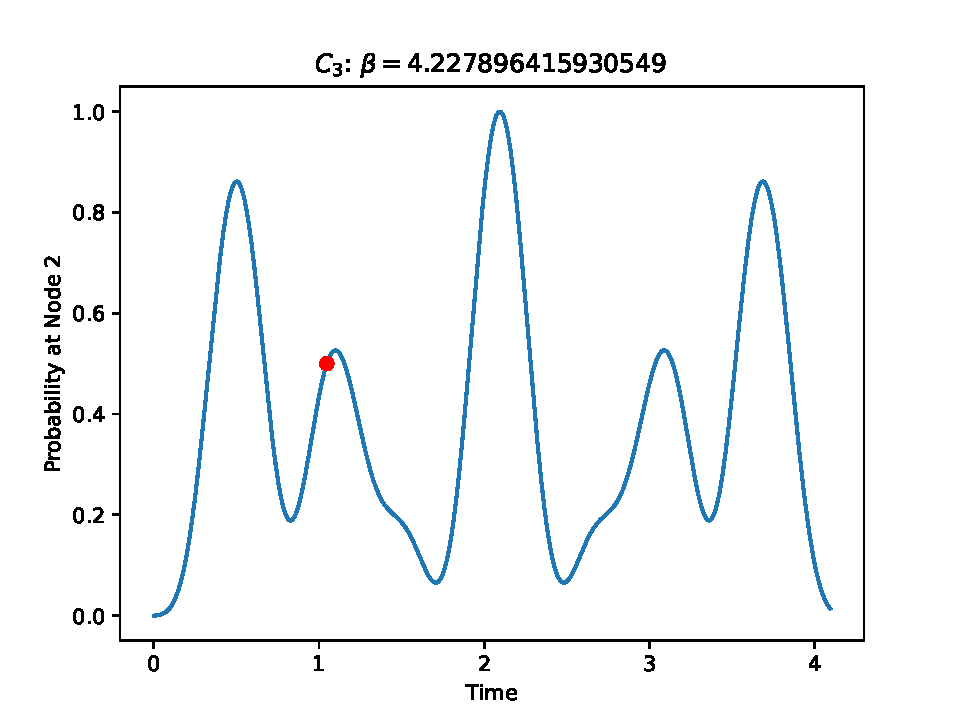
\includegraphics[width=0.7\textwidth]{c_3 (5).pdf}
\end{center}
\begin{displaymath}
    t=t'=\frac{\pi}{3}
\end{displaymath}
\begin{center}
    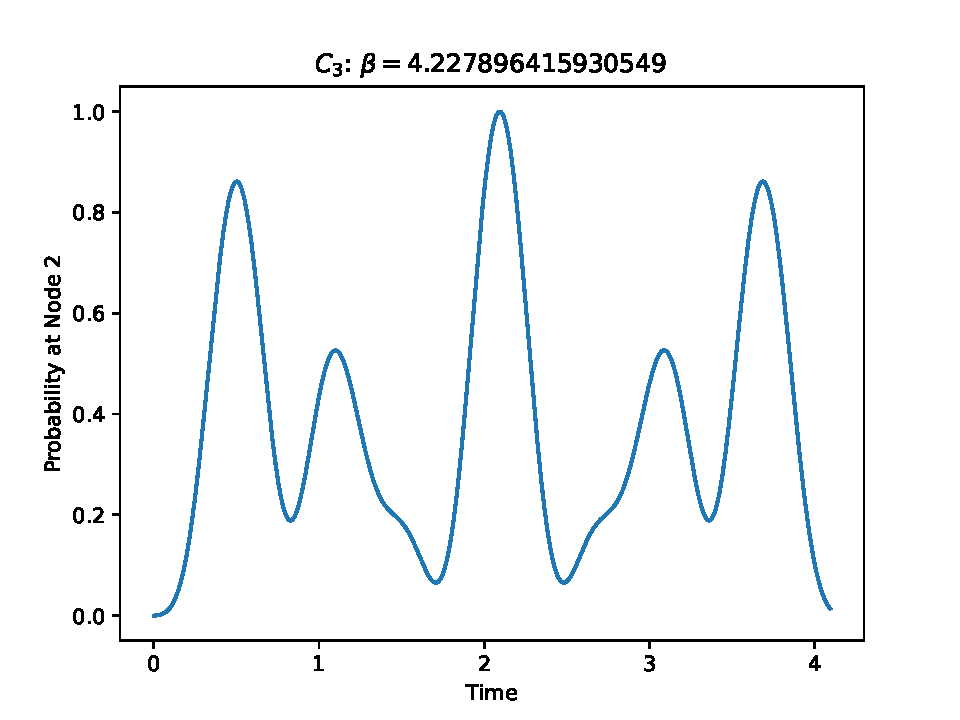
\includegraphics[width=0.7\textwidth]{c_3 (6).pdf}
\end{center}
\begin{displaymath}
    t=\frac{2\pi}{3}
\end{displaymath}
The second step appears to be unnecessary in this family.
\section{C$_3$ Node 1 $\rightarrow$ Node 3 PST}
\begin{center}
    \begin{tikzpicture}
    % Draw nodes
    \node[circle, draw, fill=white, minimum size=1cm] (1) at (0,1.5) {1};
    \node[circle, draw, fill=white, minimum size=1cm] (2) at (2.6,-1.5) {2};
    \node[circle, draw, fill=white, minimum size=1cm] (3) at (-2.6,-1.5) {3};
    
    % Draw connections
    \draw[-] (1) -- (2) node[midway, right] {$1$};
    \draw[-] (2) -- (3) node[midway, below] {$\alpha$};
    \draw[-] (3) -- (1) node[midway, left] {$\beta$};
    
    % Labels
    \node[below] at (1) {};
    \node[below] at (2) {};
    \node[below] at (3) {};
\end{tikzpicture}
\end{center}
\begin{center}
    \begin{tikzpicture}
    % Draw nodes
    \node[circle, draw, fill=white, minimum size=1cm] (1) at (0,1.5) {1};
    \node[circle, draw, fill=white, minimum size=1cm] (2) at (2.6,-1.5) {2};
    \node[circle, draw, fill=white, minimum size=1cm] (3) at (-2.6,-1.5) {3};
    
    % Draw connections
    \draw[-] (1) -- (2) node[midway, right] {$1$};
    \draw[-] (2) -- (3) node[midway, below] {$\alpha$};
    \draw[-] (3) -- (1) node[midway, left] {$-\beta$};
    
    % Labels
    \node[below] at (1) {};
    \node[below] at (2) {};
    \node[below] at (3) {};
\end{tikzpicture}
\end{center}
\subsection{Two-Step isn't Useless!!!}
\begin{center}
    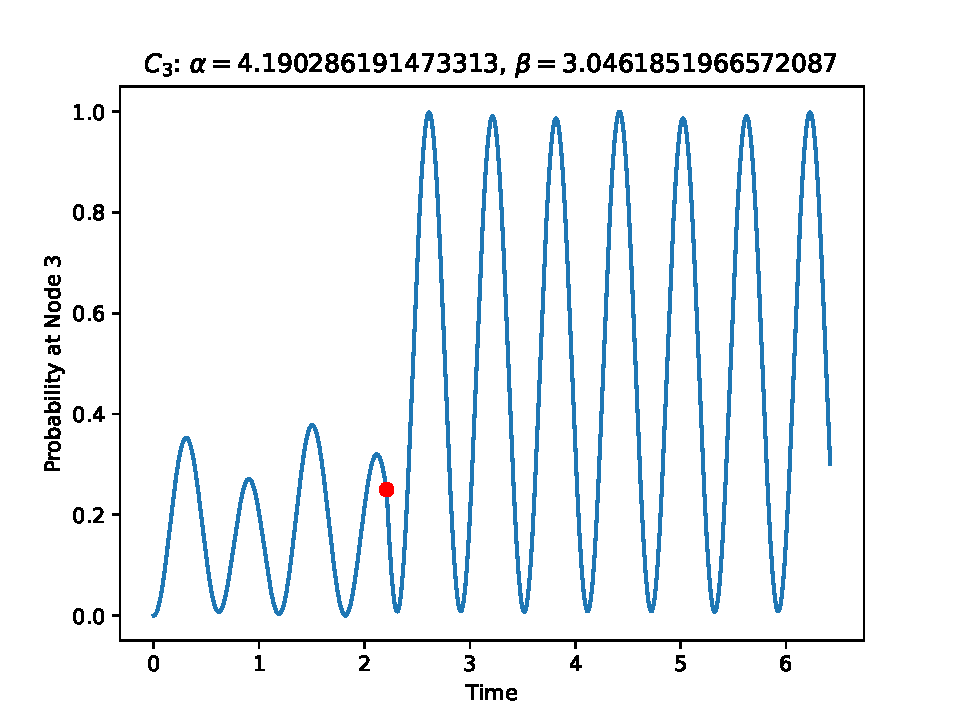
\includegraphics[width=0.7\textwidth]{c_3 (7).pdf}
\end{center}
\begin{displaymath}
    t=t'=2.210153548
\end{displaymath}
\begin{center}
    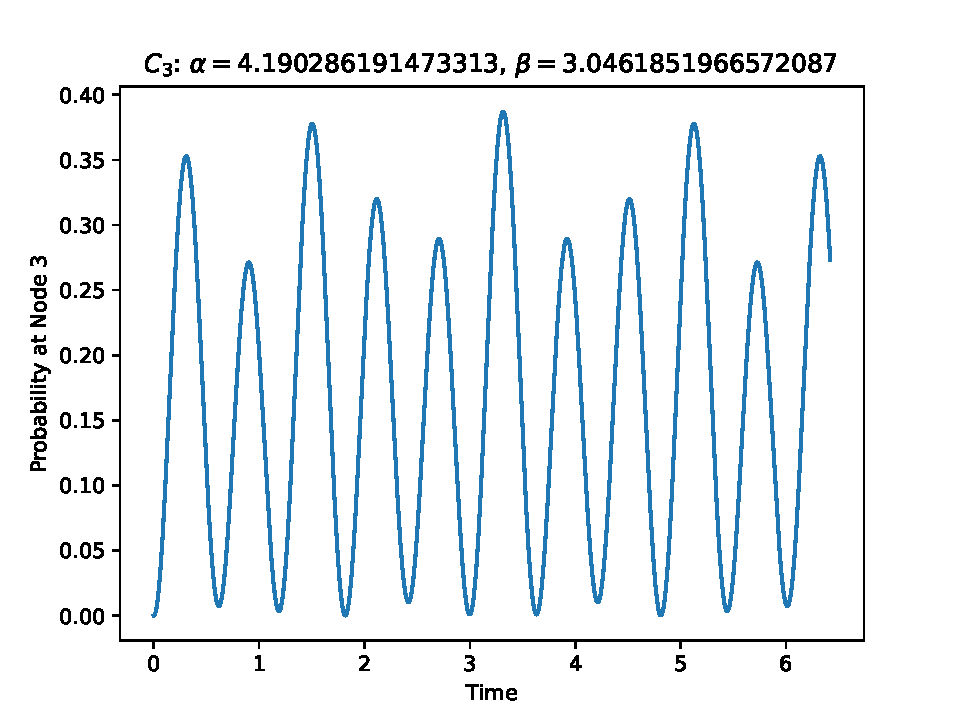
\includegraphics[width=0.7\textwidth]{c_3 (8).pdf}
\end{center}
\begin{displaymath}
    t=4.420307096
\end{displaymath}
\begin{center}
    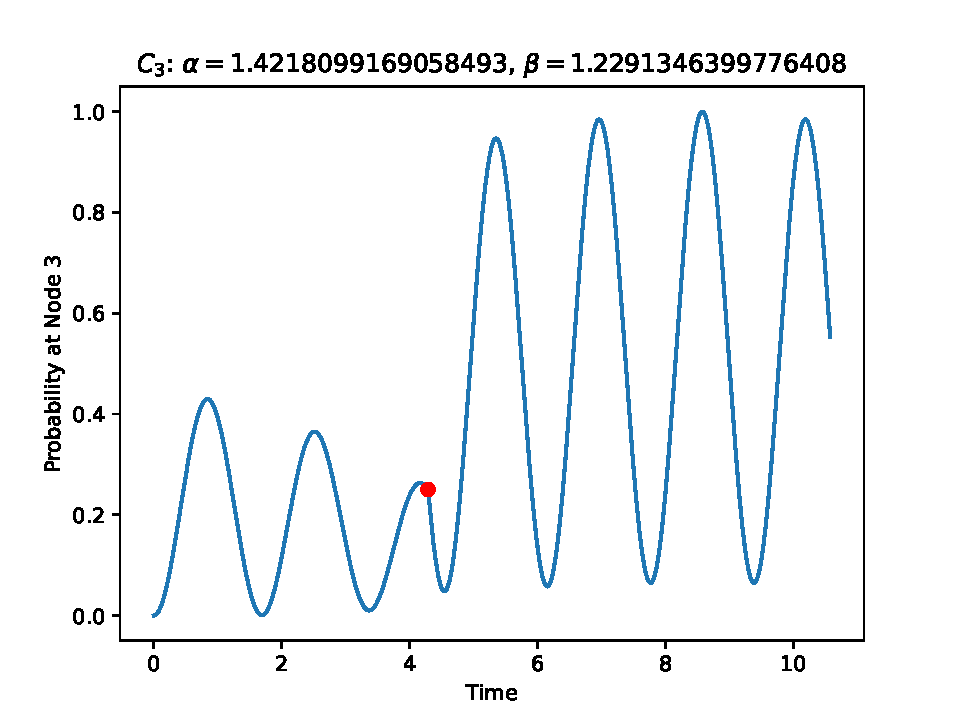
\includegraphics[width=0.7\textwidth]{c_3 (9).pdf}
\end{center}
\begin{displaymath}
    t=t'=4.288203328
\end{displaymath}
\begin{center}
    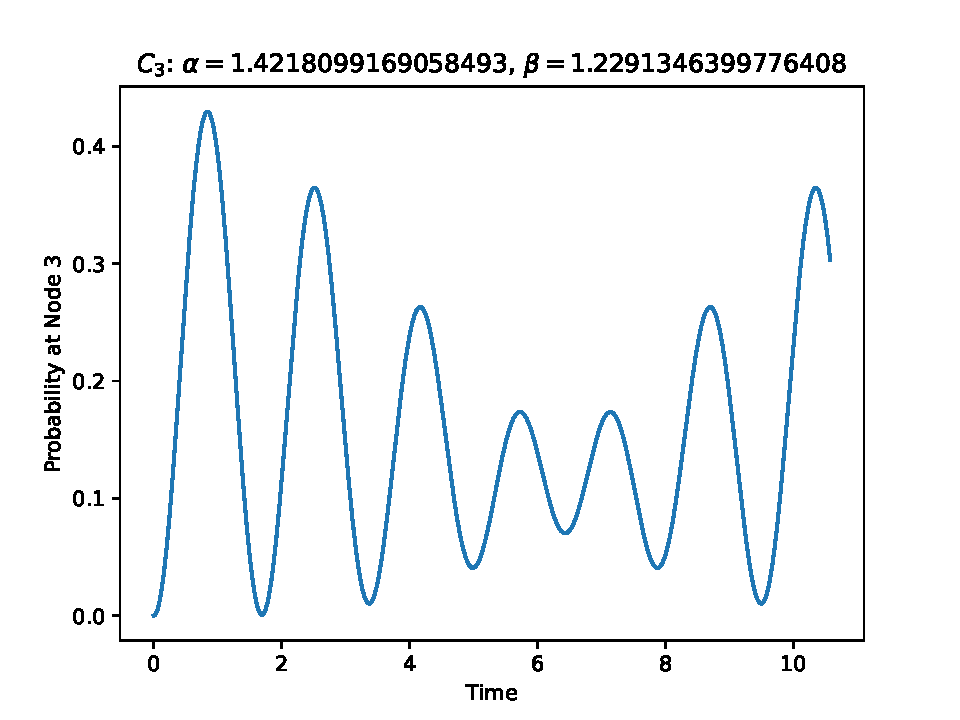
\includegraphics[width=0.7\textwidth]{c_3 (10).pdf}
\end{center}
\begin{displaymath}
    t=8.576406656
\end{displaymath}
\begin{center}
    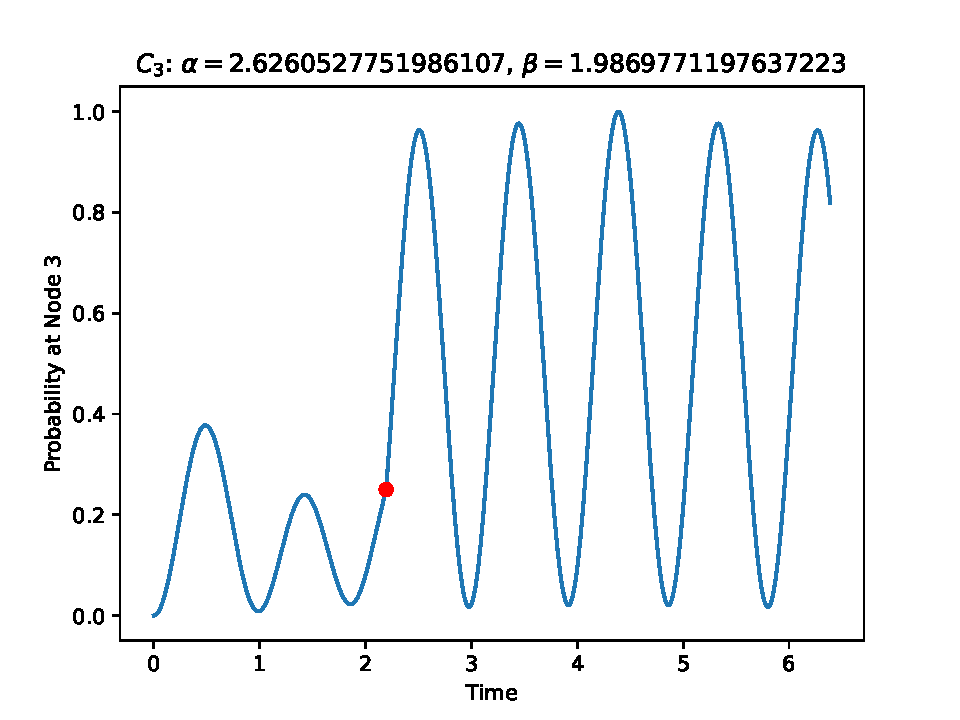
\includegraphics[width=0.7\textwidth]{c_3 (11).pdf}
\end{center}
\begin{displaymath}
    t=t'=2.19420324
\end{displaymath}
\begin{center}
    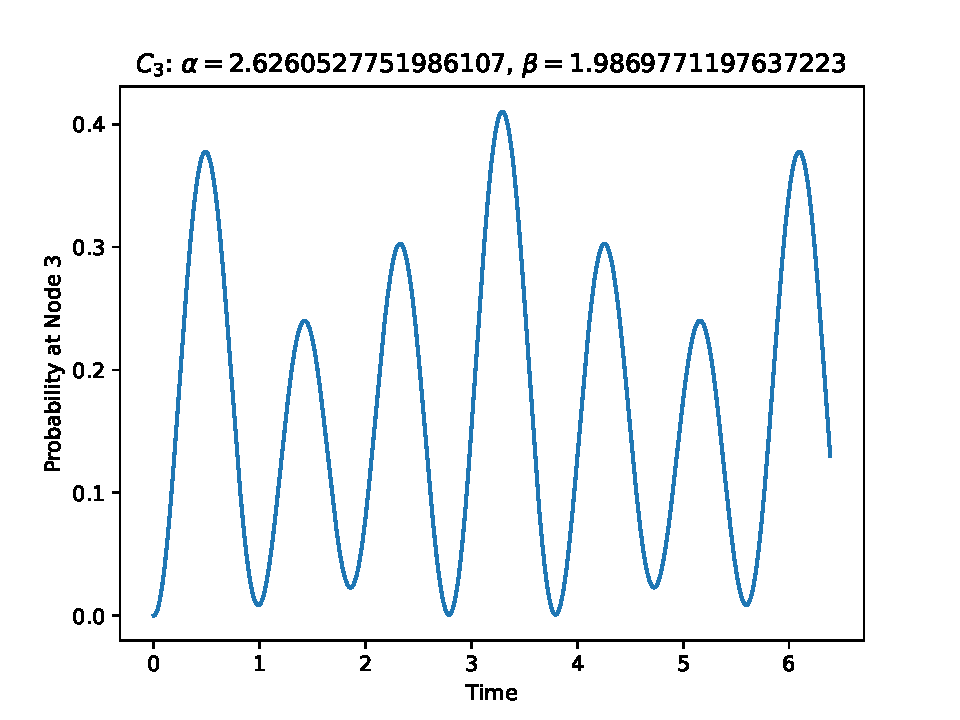
\includegraphics[width=0.7\textwidth]{c_3 (12).pdf}
\end{center}
\begin{displaymath}
    t=4.38840648
\end{displaymath}
When I was working on P$_4$, I got many results on asymmetric edge weights at first, but I thought they were all PGST and ignored them. Now thinking back, two-step PST might be the only way to achieve perfect fidelity on asymmetric graphs.
\newpage
\subsection{Checking for Periodicity in One-Step PST}
\begin{center}
    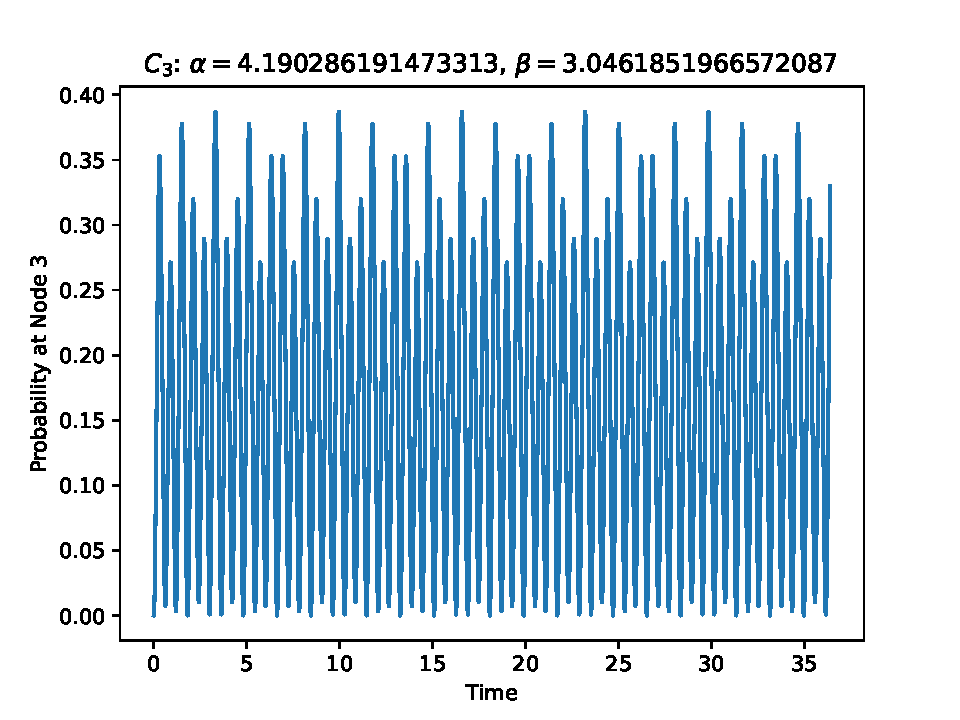
\includegraphics[width=0.7\textwidth]{periodic (3).pdf}
\end{center}
\begin{center}
    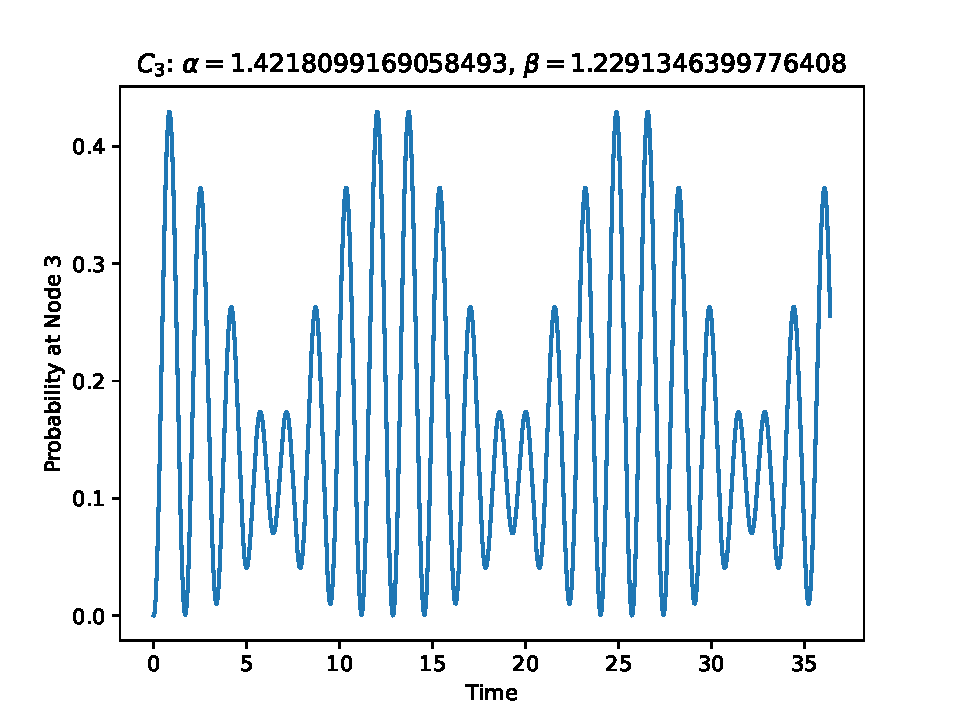
\includegraphics[width=0.7\textwidth]{periodic (2).pdf}
\end{center}
\begin{center}
    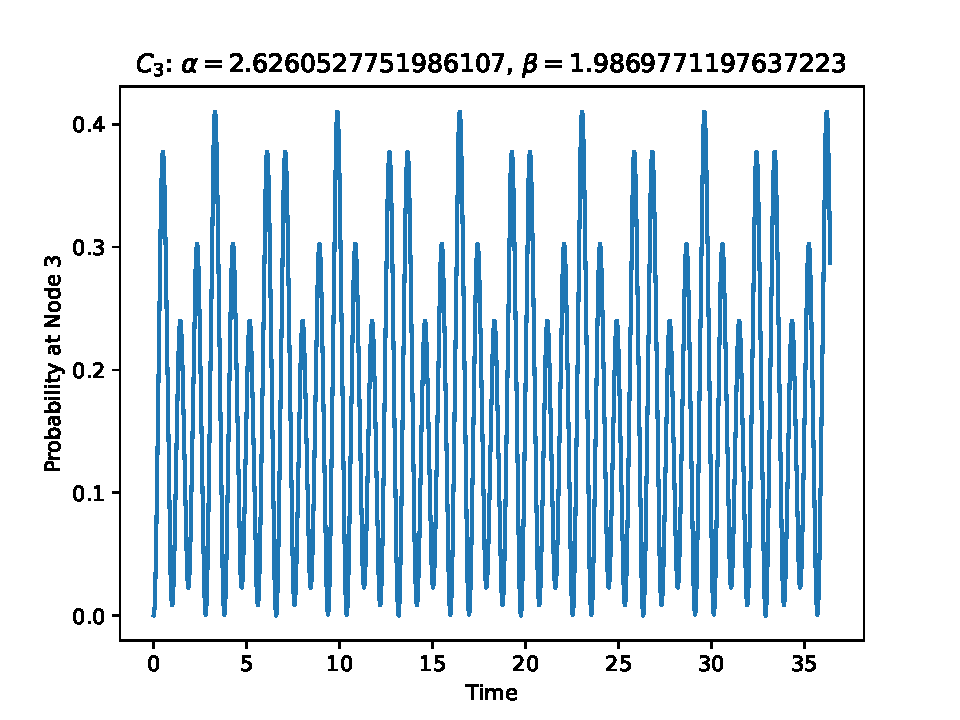
\includegraphics[width=0.7\textwidth]{periodic (1).pdf}
\end{center}
I think it is safe to say that without the second step, the fidelity never reach 1, not even close.
\newpage
\section{Appendix}
\subsection{Proof of Eq.~\ref{eq:exponential spectral decomposition}}
We know that
\begin{equation}
    \label{eq:expansion}
    e^x=\sum_{n=0}^\infty\nicefrac{x^n}{n!}
\end{equation}
Therefore, by $\langle u_n|u_m\rangle=\delta_{nm}$, $e^{-\nicefrac{iHt}{\hbar}}$ can be rewritten as
\begin{align}
    e^{-\frac{i H t}{\hbar}} &= \sum_{n=0}^{\infty} \frac{1}{n!} \left(-\frac{i H t}{\hbar}\right)^n\nonumber\\
    &= \sum_{n=0}^{\infty} \frac{1}{n!} \left(-\frac{i t}{\hbar} \sum_m \lambda_m |u_m\rangle \langle u_m| \right)^n\nonumber\\
    &= \sum_{n=0}^{\infty} \frac{1}{n!} \sum_m \left(-\frac{i \lambda_m t}{\hbar}\right)^n |u_m\rangle \langle u_m|\nonumber\\
    &= \sum_m \left( \sum_{n=0}^{\infty} \frac{1}{n!} \left(-\frac{i \lambda_m t}{\hbar}\right)^n \right) |u_m\rangle \langle u_m|\nonumber\\
    &= \sum_m e^{-\frac{i \lambda_m t}{\hbar}} |u_m\rangle \langle u_m|\nonumber\\
    &= \sum_n e^{-\frac{i \lambda_n t}{\hbar}} |u_n\rangle \langle u_n|
\end{align}
\subsection{Equation to be Solved}
\begin{equation}
    \begin{pmatrix}
        0\\
        0\\
        0\\
        1
    \end{pmatrix}=e^{-\nicefrac{iH't}{\hbar}}\left[e^{-\nicefrac{iHt}{\hbar}}\begin{pmatrix}
        1\\
        0\\
        0\\
        0
    \end{pmatrix}\right]
\end{equation}
where
\begin{align}
    H=&\begin{pmatrix}
        0&1&0&0\\
        1&0&\nicefrac{6}{\sqrt{7}}&0\\
        0&\nicefrac{6}{\sqrt{7}}&0&1\\
        0&0&1&0
    \end{pmatrix}\\
    H=&\begin{pmatrix}
        0&-1&0&0\\
        -1&0&\nicefrac{6}{\sqrt{7}}&0\\
        0&\nicefrac{6}{\sqrt{7}}&0&-1\\
        0&0&-1&0
    \end{pmatrix}
\end{align}
\end{document}
